\documentclass[]{elsarticle}
\setlength{\marginparwidth}{0.5in}
\usepackage{amsmath,amssymb,amsthm,mathtools,booktabs,array,tikz,pifont,graphicx}
\input FJHDef.tex

\DeclareMathOperator{\lin}{lin}
\DeclareMathOperator{\up}{up}
\DeclareMathOperator{\lo}{lo}
\DeclareMathOperator{\fix}{non}
\DeclareMathOperator{\err}{err}
\newcommand{\herr}{\widehat{\err}}

\newtheorem{theorem}{Theorem}
\newtheorem{prop}[theorem]{Proposition}
\newtheorem{lem}{Lemma}
\newtheorem{cor}{Corollary}
\theoremstyle{definition}
\newtheorem{algo}{Algorithm}
\newtheorem{condit}{Condition}
%\newtheorem{assump}{Assumption}
\theoremstyle{remark}
\newtheorem{rem}{Remark}


\journal{Journal of Complexity}

\begin{document}

\begin{frontmatter}

\title{The Complexity of Deterministic Guaranteed Automatic Algorithms}
\author{Yuhan Ding}
\author{Nicholas Clancy}
\author{Caleb Hamilton}
\author{Fred J. Hickernell}
\author{Yizhi Zhang}
\address{Room E1-208, Department of Applied Mathematics, Illinois Institute of Technology,\\ 10 W.\ 32$^{\text{nd}}$ St., Chicago, IL 60616}
\begin{abstract} Automatic numerical algorithms are widely used in practice.  An algorithm that is automatic attempts to provide an approximate solution that differs from the true solution by no more than a user-specified tolerance, $\varepsilon$. Furthermore, the computational effort required is typically determined adaptively by the algorithm based on function data, e.g., function values.  Ideally, the computational cost should match the difficulty of the problem.  Unfortunately, most automatic algorithms lack rigorous guarantees, i.e., sufficient conditions on the input function that ensure the success of the algorithm. 

This article establishes a framework for providing rigorous guarantees for automatic, adaptive algorithms. Sufficient conditions for success and upper bounds on the computational cost are provided in Theorems \ref{TwoStageDetermThm} and \ref{MultiStageThm}.  Lower bounds on the complexity of the problem are given in Theorem \ref{complowbd} and conditions are given under which the proposed algorithms attain those lower bounds in Corollary \ref{optimcor}. These general theorems are illustrated with automatic algorithms for univariate numerical integration and function recovery using linear interpolation.  The key observation is that the error analysis should be done for \emph{cones} of input functions rather than balls. The existing literature contains certain cautions about the usefulness and reliability of automatic algorithms.  The theory presented here does not share the assumptions on which those concerns are based, rendering those concerns irrelevant.
\end{abstract}

\begin{keyword}
adaptive \sep automatic \sep cones \sep function recovery \sep integration \sep quadrature
%% keywords here, in the form: keyword \sep keyword

\MSC[2010] 65D05 \sep 65D30 \sep 65G20
%% MSC codes here, in the form: \MSC code \sep code
%% or \MSC[2008] code \sep code (2000 is the default)

\end{keyword}
\end{frontmatter}

\section{Introduction}

Numerical algorithms for evaluating many elementary and special functions of real variables reliably provide answers to machine precision with minimal user input.  For example, the MATLAB \cite{MAT7.12} algorithms
\[
{\tt cos, sin, exp, log, airy, besselj, gamma, gammainc, ellipj, erf,} \text{ and } {\tt  erfinv}
\] 
all automatically use the right number of terms in a suitable expansion needed to provide the corresponding function value with $15$ significant digit accuracy. The only exceptions are cases of unavoidable round-off error, e.g., 
\[
{\tt cos(1e47*pi)= -5.432862626006405e-01},
\]
whereas the correct answer is {\tt 1}.

We also want algorithms that require minimal user input to obtain the desired answer for more complex numerical problems, e.g., integration and function recovery, where the inputs are functions rather than real variables.  Namely, we want \emph{algorithms with the following properties:}
\begin{description}
\item[Guaranteed]--- the errors in the answers provided must be no greater than the user-specified \emph{error tolerance}, $\varepsilon$.
\item[Automatic]--- the computational effort required depends on $\varepsilon$, but \emph{does not require additional user input} beyond a routine for providing function data.
\item[Adaptive]--- the computational effort depends on the input function, specifically, on the difficulty of the problem (size of the input function) \emph{as inferred from function data, not specified a priori}.
\item[Optimal]--- the computational cost of the algorithm, as $\varepsilon \to 0$, asymptotically matches the computational complexity of the problem, i.e., the computational cost of the best possible algorithm.  The computational cost as a function of the unknown problem difficulty is asymptotically the same as that of the best algorithm possible \emph{even if the problem difficulty were known a priori}.
\item[Tunable]--- parmeters defining the algorithm can be adjusted to change the algorithm's robustness, the maximum allowable computational cost budget, etc.  These parameters are intended to be changed only occasionally, as opposed to inputs, which may change each time that the algorithm is called.
\end{description}
The checklist in Figure \ref{fig:checklist} rates some common algorithms currently in use and those proposed here against these five criteria.  As noted, the existing algorithms nearly all fail to meet one or more of these criteria.  Here we present a general framework for constructing algorithms that satisfy all of the above criteria.  We also present two concrete examples, namely, univariate integration via the composite trapezoidal rule and univariate function recovery via linear splines.

Automatic quadrature algorithms such as MATLAB's {\tt quad} and {\tt quadgk} \cite{MAT7.12} and those in the NAG Library \cite{NAG23} work well for many cases in practice, but they do not have rigorous guarantees of success.  The Chebfun toolbox in MATLAB \cite{TrefEtal12} approximates functions by Chebyshev polynomial expansions and uses those expansions to approximate integrals, solve differential equations, etc. Chebfun also works well for many cases, but has no guarantees.  All of these algorithms are adaptive.  The degree to which they are tunable varies.

\begin{figure}[ht]
\centering 
\begin{tabular}{r>{\centering}b{2.8cm}>{\centering}b{2.8cm}>{\centering}b{2.8cm}}
& MATLAB, NAG, and Chebfun
& Algorithm in Figure \ref{fig:NonadaptAlgo}
& Algorithm in Figure \ref{fig:AdaptAlgo} \tabularnewline
\toprule
Guaranteed & & \ding{51} & \ding{51}  \tabularnewline
Automatic & \ding{51} & \ding{51} & \ding{51} \tabularnewline
Adaptive & \ding{51} & & \ding{51} \tabularnewline
Optimal & & \ding{51} & \ding{51} \tabularnewline
Tunable & ? & \ding{51} & \ding{51} 
\end{tabular}
\caption{Check list of desired features for an algorithm. \label{fig:checklist}}
\end{figure}

Most existing theory for numerical problems of interest starts with a Banach space, $\cf$, of input functions defined on some set $\cx$, and having a semi-norm, $\norm[\cf]{\cdot}$.  The definition of $(\cf,\norm[\cf]{\cdot})$ contains assumptions about smoothness, periodicity or other qualities of the input functions.  The mathematical problem of interest is defined by a \emph{solution operator} $S:\cf \to \ch$, where $\ch$ is some other Banach space with its norm $\norm[\ch]{\cdot}$.  For integration, $\ch=\reals$, and for function approximation, $\ch$ is some superset of $\cf$, for example, $\cl_{\infty}(\cx)$. Given this set-up, one often finds an algorithm, $A_n$, with computational cost $n$, that provides an approximate solution whose error can be bounded as
\begin{subequations} \label{traditionerr}
\begin{equation} \label{traditionerra}
\norm[\ch]{S(f)-A_n(f)} \le \frac{C_{\up} \norm[\cf]{f}}{n^p}, \quad n \in \naturals,
\end{equation}
where $C_{\up}$ and $p$ are some known constants.  It is necessarily assumed that the algorithm is exact if the semi-norm of the input function vanishes, i.e., $S(f)=A_n(f)$ if $\norm[\cf]{f}=0$.  Error bound \eqref{traditionerra} allows one to compute an approximation that differs from the true solution by no  more than $\varepsilon$, provided that the input functions lie inside a {\em ball}, i.e., 
\begin{gather}
\sup_{f \in \cb_{\sigma}} \norm[\ch]{S(f)-A_n(f)} \le \varepsilon, \qquad 
\cb_\sigma=\{ f \in \cf : \norm[\cf]{f} \le \sigma\}, \label{balldef} \\
\label{costupbd}
n=\cost(A_n) = \left \lceil \left(\frac{C_{\up}\sigma}{\varepsilon}\right)^{1/p} \right \rceil.
\end{gather}
\end{subequations}
Furthermore, there is a simple formula for the computational cost required to meet the error tolerance, $\varepsilon$, for all functions in the ball of radius $\sigma$.

Figure \ref{fig:NonadaptAlgo} provides a diagram of an automatic algorithm based on these ideas.  The parameter $\sigma$ is considered to be fixed initially by the user or algorithm designer, but then left unchanged each time the algorithm is called.  Once $\sigma$ is fixed, the algorithm only requires as input the error tolerance and a routine for evaluating the function at any point desired.  This algorithm is guaranteed.  It is optimal if any algorithm satisfying the error criterion above must have a cost of at least $\Order((\sigma/\varepsilon)^{1/p})$.  However, this algorithm is not adaptive.  The computational cost does not depend on function data, but is determined purely by the input $\varepsilon$ and the parameter $\sigma$.  In the terminology of information-based complexity theory, the computational cost depends on global information but not local information \cite[p.\ 11--12]{TraWer98}.

\begin{figure}[h]
\centering
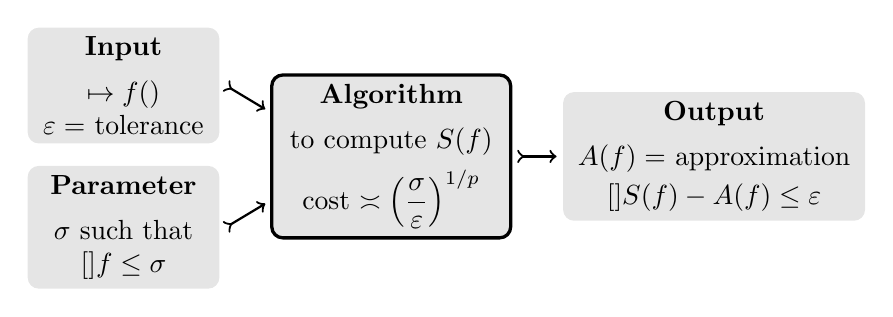
\begin{tikzpicture}
[auto,
block/.style ={rectangle, very thick, fill=black!10, align=center, rounded corners, minimum height=3em}]
%[auto,
%block/.style ={rectangle, very thick, fill=red!15, align=center, rounded corners, minimum height=3em}]
\draw (1.1,0.9) node[block, text width=2.2cm] {\parbox{2.2cm}{\centering {\bf Input}\\[1ex]
$\vx \mapsto f(\vx)$\\ 
$\varepsilon = $ tolerance}};
\draw (1.1,-0.9) node[block, text width=2.2cm] {\parbox{2.2cm}{\centering {\bf Parameter}\\[1ex]
$\sigma$ such that $\norm[\cf]{f} \le \sigma$}};
\draw (4.5,0) node[block, draw=black, text width=2.8cm] {\parbox{2.8cm}{\centering{\bf Algorithm}\\[1ex] to compute $S(f)$ \\[1ex]
%\draw (4.5,0) node[block, draw=red, text width=2.8cm] {\parbox{2.8cm}{\centering{\bf Algorithm}\\[1ex] to compute $S(f)$ \\[1ex]
cost $\displaystyle \asymp \left(\frac{\sigma}{\varepsilon}\right)^{1/p}$}};
\draw (8.6,0) node[block, text width=3.6cm] {\parbox{3.6cm}{\centering {\bf Output}\\[1ex] $A(f) = $ approximation \\[0.5ex] $\norm[\ch]{S(f)-A(f)} \le \varepsilon$}};
\draw [>->,thick] (2.4,0.9) -- (2.9,0.6);
\draw [>->,thick] (2.4,-0.9) -- (2.9,-0.6);
\draw [>->,thick] (6.1,0) -- (6.6,0);
\end{tikzpicture}
\caption{Diagram of a guaranteed, non-adaptive algorithm. \label{fig:NonadaptAlgo}}
\end{figure}

The norm $\norm[\cf]{f}$ may be thought of as the \emph{difficulty of the problem}.  In practice, it is difficult to know a priori how large $\norm[\cf]{f}$ is, so having to fix the parmeter $\sigma$ in advance is a practical drawback of the algorithm in Figure \ref{fig:NonadaptAlgo}.  Moreover, since the computational cost of this algorithm depends on $\sigma$, not $\norm[\cf]{f}$, the cost does not decrease if $\norm[\cf]{f}$ is drastically smaller than $\sigma$.  

Adaptive algorithms use function data to try to bound $\norm[\cf]{f}$ or estimate $\norm[\ch]{S(f)-A_n(f)}$, so that the computational cost can be adjusted accordingly. Unfortunately, the bounds on $\norm[\cf]{f}$ and the estimates of $\norm[\ch]{S(f)-A_n(f)}$ are typically heuristic or valid only in the limit of $n \to \infty$.  Thus, these approaches are not guaranteed to provide the answer to within the specified error tolerance for finite $n$.  Here we show how to construct a \emph{rigorous} upper bound on $\norm[\cf]{f}$ from data, that then leads to a guaranteed automatic and adaptive algorithm.  

The key idea is to consider functions lying in a \emph{cone} instead of a ball.  Let $\cg$ be some superspace of $\cf$ with a weaker semi-norm, and define the cone
\begin{equation} \label{conedef}
\cc_{\tau}=\{f \in \cf : \norm[\cf]{f} \le \tau \norm[\cg]{f} \}.
\end{equation}
Functions inside the cone may have large norms, but their $\cg$-semi-norm can be estimated with reasonable effort.  Our approach to obtaining a reliable approximation to the true solution, $S(f)$, based on on function data is outlined here in simplified form:
\begin{itemize}
\item Since the $\cg$-semi-norm is weaker than the $\cf$-semi-norm, it can be approximated by some algorithm $G(f)$, with $0\le \norm[\cg]{f}-G(f) \le C_1\norm[\cf]{f}$ for some known $C_1$.  By choosing sufficiently many function data, one may make $C_1$ as small as desired, and indeed it must be made smaller than $1/\tau$.

\item The definition of the cone in \eqref{conedef} implies that $\norm[\cg]{f} \le G(f)/(1 - \tau C_1)$.

\item Applying the cone condition again leads to an upper bound on the $\cf$-semi-norm, namely,  $\norm[\cf]{f} \le \tau G(f)/(1 - \tau C_1)$.

\item This data-driven upper bound on $\norm[\cf]{f}$ can be used with \eqref{costupbd} to guarantee that the error tolerance will be met using $A_n$ with
\[
n=\cost(A_n)\le \left \lceil\left(\frac{ C_{\up}\tau G(f)}{\varepsilon(1 - \tau C_1)}\right)^{1/p} \right \rceil.
\]

\item Furthermore, since $G(f)$ never overestimates the $\cg$-semi-norm of $f$, one can be assured that the above criterion will be met for 
\[
n=\cost(A_n)\le \left \lceil\left(\frac{ C_{\up}\tau \norm[\cg]{f}}{\varepsilon(1 - \tau C_1)}\right)^{1/p} \right \rceil.
\]
Given that $\norm[\cf]{f} = \tau \norm[\cg]{f}$ for some $f$, the cost of this algorithm as $\varepsilon \to 0$ is asymptotically the same as if one did know $\norm[\cf]{f}$ in advance.

\item On top of the above analysis, we allow for a maximum computational cost budget, $N_{\max}$, that allows the user to specify how long he or she is willing to wait for an answer.

\end{itemize} 
Figure \ref{fig:AdaptAlgo} is a diagram of the automatic algorithm just outlined.

\begin{figure}[h]
\centering
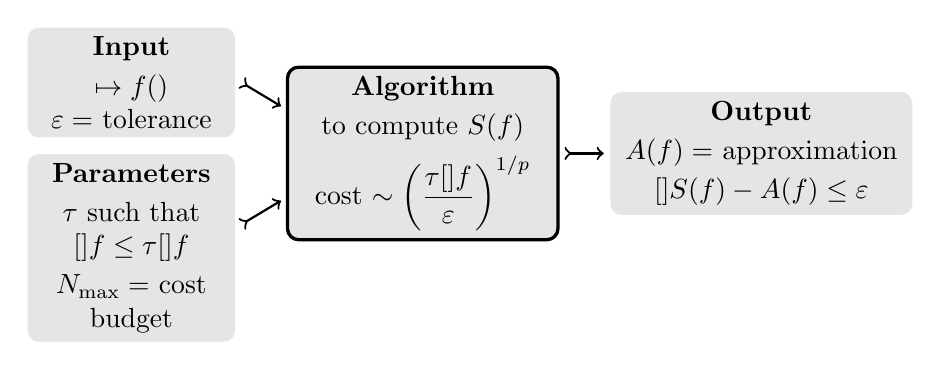
\begin{tikzpicture}
[auto,
block/.style ={rectangle, very thick, fill=black!10, align=center, rounded corners, minimum height=3em}]
%[auto,
%block/.style ={rectangle, very thick, fill=red!15, align=center, rounded corners, minimum height=3em}]
\draw (1.2,0.9) node[block, text width=2.4cm] {\parbox{2.4cm}{\centering{\bf Input}\\[0.5ex] 
$\vx \mapsto f(\vx)$\\ 
$\varepsilon = $ tolerance}};
\draw (1.2,-1.2) node[block, text width=2.4cm] {\parbox{2.4cm}{\centering{\bf Parameters}\\[0.5ex] 
$\tau$ such that $\norm[\cf]{f} \le \tau\norm[\cg]{f}$ \\[0.5ex] $N_{\max} = $ cost budget}};
\draw (4.9,0) node[block, draw=black, text width=3.2cm] {\parbox{3.2cm}{\centering{\bf Algorithm}\\[0.5ex] to compute $S(f)$ \\[1ex]
%\draw (5.1,0) node[block, draw=red, text width=3.2cm] {\parbox{3.2cm}{\centering{\bf Algorithm}\\[1ex] to compute $S(f)$ \\[1ex]
cost $\displaystyle \sim \left(\frac{\tau\norm[\cg]{f}}{\varepsilon}\right)^{1/p}$ }};
\draw (9.2,0) node[block, text width=3.6cm] {\parbox{3.6cm}{\centering{\bf Output}\\[0.5ex] $A(f) = $ approximation \\[0.5ex] $\norm[\ch]{S(f)-A(f)} \le \varepsilon$}};
\draw [>->,thick] (2.6,0.9) -- (3.1,0.6);
\draw [>->,thick] (2.6,-0.9) -- (3.1,-0.6);
%\draw [>->,thick] (2.6,0) -- (3.1,0);
\draw [>->,thick] (6.7,0) -- (7.2,0);
\end{tikzpicture}
\caption{Diagram of a guaranteed, adaptive, automatic algorithm. \label{fig:AdaptAlgo}}
\end{figure}

Section \ref{integsec} presents a concrete example of this approach for the problem of computing the integral $\int_0^1 f(x) \, \dif x$ for all integrands whose second derivatives are absolutely integrable, i.e., $\norm[\cf]{f}=\norm[1]{f''}$.  The trapezoidal rule computes an approximation with error no greater than $\varepsilon$ using $\Theta(\sqrt{\norm[1]{f''}/\varepsilon})$ function values.  However, except for relatively simple integrands, $\norm[1]{f''}$ is unknown in practice.  One may instead estimate $\norm[1]{f'}$ by the one-norm of the derivative of the piecewise linear spline for $f$.  The error of approximating $\norm[1]{f'}$ in this way can be bounded rigorously in terms of $\norm[1]{f''}$.  Fixing the parameter $\tau > 1$, and assuming that $\norm[1]{f''} \le \tau \norm[1]{f'}$  (the cone condition), then the reliable numerical upper bound on $\norm[1]{f'}$ can be used as a surrogate for $\norm[1]{f''}$.  This leads to a guaranteed, automatic (adaptive) algorithm for approximating the integral to the desired accuracy with a computational cost that is $\Theta(\sqrt{\tau \norm[1]{f'}/\varepsilon})$, where $\norm[1]{f'}$ is unknown a priori.  Here $\tau$ represents a minimum sample size, and $1/\tau$ represents a length scale of for possible spikes that one is willing to ignore.

This article starts with the general setting and then moves to two concrete cases.  Section \ref{probdefsec} lays out the problems to be solved.  Section \ref{NonAdaptsec} defines non-adaptive algorithms, their costs, and the complexities of numerical problems for which non-adpative algorithms are suited.  The algorithm diagrammed in Figure \ref{fig:NonadaptAlgo} is essentially this kind of algorithm.  Non-adaptive algorithms are the building blocks for adaptive algorithms.  Adaptive algorithms, their costs, and the complexity of problems defined on cones of functions are introduced in Section \ref{AutoAlgsec}.  Their cost is defined in terms of the unknown, but estimated, $\cg$-semi-norm of the input function.  The problem definition here allows for a maximum computational cost budget to be imposed so that one never needs to wait an arbitrarily large time for the answer.  

Sections \ref{genthmsec} and \ref{LowBoundSec} describes the automatic algorithms in detail and provides proofs of their success for cones of input functions.  In particular, the following results are presented:
\begin{itemize}

\item Algorithm \ref{twostagedetalgo} is a two stage algorithm, where $\norm[\cg]{f}$ is bounded above once, and then this bound is used to determine the additional computational cost, $n$, so that $A_n(f)$ achieves the desired tolerance. Algorithm \ref{multistagealgo} is a multi-stage algorithm, where the algorithm, $G_n$, used to bound $\norm[\cg]{f}$, and the algorithm, $A_n$, used to approximate $S(f)$, are based on the same data. Moreover, these are embedded algorithms whose costs increase progressively according to some sequence $n_1, n_2, \ldots$.  Once the number of samples is sufficiently large so that $A_{n_i}(f)$ achieves the desired tolerance, the algorithm terminates.

\item Theorems \ref{TwoStageDetermThm} and \ref{MultiStageThm} in Section \ref{genthmsec} prove that Algorithms \ref{twostagedetalgo} and \ref{multistagealgo}, respectively, are guaranteed to produce answers to within the desired error tolerance, provided that they do not exceed the maximum cost budget.  These theorems also demonstrate that the computational costs of these algorithms do not exceed the costs of algorithms that know $\norm[\cf]{f}$ or $\norm[\cg]{f}$ a priori.

\item Theorem \ref{complowbd} in Section \ref{LowBoundSec} provides lower bounds on the computational complexity of the problems defined on cones of input functions by constructing fooling functions.  Corollary \ref{optimcor} shows that Algorithms \ref{twostagedetalgo} and \ref{multistagealgo} are optimal if the non-adaptive algorithms on which they are based are optimal for problems defined on balls of input functions.

\end{itemize}

Section \ref{integsec} illustrates the general theorems in Sections \ref{genthmsec} and \ref{LowBoundSec} for the univariate integration problem.  An explicit automatic algorithm based on the trapezoidal rule is presented and its success and optimality are proved.  Section \ref{approxsec}  considers function approximation with a analogous results.  Common concerns about automatic and adaptive algorithms are answered in Section \ref{overcomesec}. The article ends with several suggestions for future work.

\section{General Problem Definition} \label{probdefsec}

\subsection{Problems and Algorithms} The function approximation, integration, or other problem to be solved is defined by a \emph{solution operator} $S:\cf \to \ch$, where $\cf$ is a Banach space of possible input functions defined on $\cx$ with semi-norm $\norm[\cf]{\cdot}$, and $\ch$ is some other Banach of possible outputs or solutions with norm $\norm[\ch]{\cdot}$. The solution operator is assumed to have a scale property, i.e., 
\[
S(cf) = cS(f) \qquad \forall c\ge 0.
\]
Examples include the following:
\begin{align*}
\text{Integration:} \quad & S(f) = \int_{\cx} f(\vx) \, \rho(\vx) \, \dif \vx, \quad \rho \text{ is fixed,}\\
\text{Function Recovery:} \quad & S(f) = f, \\
\text{Poisson's Equation:} \quad & S(f) = u, \quad \text{where } \begin{array}{c} -\Delta u(\vx) = f(\vx), \ \vx \in \cx, \\ u(\vx)=0 \ \forall \vx \in \partial \cx, \text{ and}\end{array} \\
\text{Optimization:} \quad & S(f) = \min_{\vx \in \cx} f(\vx).
\end{align*}
The first three examples above are linear problems, which automatically have the scale property for $S$, but the last example is a nonlinear problem, which nevertheless also has the scale property.

The goal is to find an algorithm $A:\cf \to \ch$ for which $S(f) \approx A(f)$. Following the definition of algorithms described in \cite[Section 3.2]{TraWasWoz88}, the algorithm takes the form of some function of data derived from the input function:
\begin{equation}
\label{algoform}
A(f) =  \phi(\vL(f)), \quad \vL(f) = \left(L_1(f), \ldots, L_m(f)\right) \qquad \forall f \in \cf.
\end{equation}
Here the $L_i \in \Lambda$ are real-valued functions defined on $\cf$ with the following scale property:
\begin{equation}
\label{dataassump}
L(cf) = cL(f) \qquad \forall f \in \cf, \ c \in \reals, \ L \in \Lambda.
\end{equation}
One popular choice for $\Lambda$ is the set of all function values, $\Lambda^{\std}$, i.e., $L_i(f) = f(\vx_i)$ for some $\vx_i \in \cx$.  Another common choice is the set of all bounded linear functionals, $\Lambda^{\lin}$.  In general, $m$ may depend on $f$ and the choice of $L_i$ may depend on $L_1(f), \ldots, L_{i-1}(f)$.  In this article, all algorithms are assumed to be deterministic.  There is no random element.

\subsection{Non-Adaptive Algorithms} \label{NonAdaptsec}

The set $\ca_{\fix}(\cf,\ch,S,\Lambda)$ contains algorithms as just described for which the choice of the $L_i$ and the number of function data used by the algorithm, $m$, are both assumed to be independent of the input function, i.e., these algorithms are non-adaptive.  Furthermore, any $A \in \ca_{\fix}(\cf,\ch,S,\Lambda)$ is assumed to satisfy the following scale properties:
\begin{equation}
\label{algoscale}
\vL(cf) = c \vL(f), \quad 
\phi(c\vy) = c\phi(\vy), \quad A(cf) = cA(f) \qquad \forall c \ge 0, \ \vy \in \reals^m.
\end{equation}

The cost of a non-adaptive algorithm, $A \in  \ca_{\fix}(\cf,\ch,S,\Lambda)$, is fixed and is defined as the sum of the costs of all the function data:
\begin{equation} \label{costfix}
\cost(A) = \$(\vL) = \$(L_1) + \cdots +\$(L_m),
\end{equation}
where $\$:\Lambda \to [1,\infty)$, and $\$(L)$ is the cost of acquiring the datum $L(f)$. The cost of $L$ may be the same for all $L \in \Lambda$, e.g, $\$(L)=1$.  Alternatively, the cost might vary with the choice of $L$.  E.g., if $f$ is a function of the infinite sequence of real numbers, $(x_1, x_2, \ldots)$, the cost of evaluating the function with arbitrary values of the first $d$ coordinates, $L(f)=f(x_1, \ldots, x_d, 0, 0, \ldots)$, might be $d$.  This cost model has been used by \cite{HicMGRitNiu09a,KuoEtal10a,NiuHic09a,NiuHic09b,PlaWas11a} for integration problems and \cite{Was13a,WasWoz11a,WasWoz11b} for function approximation problems.

The error of a non-adaptive algorithm $A  \in \ca_{\fix}(\cf,\ch,S,\Lambda)$ is defined  as
\begin{equation} \label{errdefworst}
\err(A,\cf,\ch,S)
= \min\{ \delta \ge 0 : \norm[\ch]{S(f) -  A(f)} \le \delta \norm[\cf]{f} \ \forall f \in \cf \},
\end{equation}
When the problem has real-valued solutions, i.e., $\ch=\reals$, one may also define a one sided error criterion:
\begin{equation}\label{errpmdefworst}
\err_{\pm}(A,\cf,\reals,S) = 
\min \{ \delta \ge 0 : \pm[S(f) -  A(f)] \le \delta \norm[\cf]{f} \ \forall f \in \cf \}. 
\end{equation}
Since $\norm[\cf]{\cdot}$ may be a semi-norm, but not a norm, a finite error in any of the above definitions assumes that the algorithm is exact, i.e., $S(f)=A(f)$, for all $f$ with $\norm[\cf]{f}=0$.

The above error criteria are normalized, meaning that the absolute error, $\norm[\ch]{S(f) -  A(f)}$ is measured with respect to the $\cf$-semi-norm of the input function. The complexity of a problem for this set of algorithms, $\ca_{\fix}(\cf,\ch,S,\Lambda)$, is defined as the cost of the cheapest algorithm that satisfies the specified error tolerance, $\varepsilon$:
\begin{multline} \label{fixcostcomplex}
\comp(\varepsilon,\ca_{\fix}(\cf,\ch,S,\Lambda)) \\
= \inf\left\{\cost(A) : \err(A,\cf,\ch,S) \le \varepsilon, \ A \in \ca_{\fix}(\cf,\ch,S,\Lambda) \right \}.
\end{multline}
Here the infimum of an empty set is defined to be $\infty$.  This means that to guarantee that $\norm[\ch]{S(f) -  A(f)} \le \varepsilon$, one needs an algorithm with a cost of at least 
\[
\comp(\varepsilon/\norm[\cf]{f},\ca_{\fix}(\cf,\ch,S,\Lambda)).
\]
This cost does not decrease as either $\varepsilon$ decreases or $\norm[\cf]{f}$ increases.

Suppose that there is a sequence of nonadaptive algorithms indexed by their cost, and which converge to the true answer:
\begin{subequations} \label{algseqdef}
\begin{gather} 
\{A_n\}_{n \in \ci}, \qquad A_n  \in \ca_{\fix}(\cf,\ch,S,\Lambda), \\
\lim_{\substack{n \to \infty\\ n \in \ci}} \err(A_n,\cf,\ch,S) = 0, \qquad \cost(A_n) = n,  
\end{gather}
\end{subequations}
where the countable, non-negative-valued index set, 
\begin{equation} \label{indexdef}
\ci=\{n_1, n_2, \ldots\} \quad \text{with } n_i < n_{i+1}, \quad \text{satisfies } \sup_i \frac{n_{i+1}}{n_i} <\infty. 
\end{equation} 
This sequence of algorithms is called \emph{optimal} for the problem $(\cf,\ch,S,\Lambda)$ if it essentially tracks the minimum cost algorithms, namely,
\begin{equation} \label{nearoptdef}
\sup_{0 < \varepsilon \le 1} \frac{\min\{n \in \ci : \err(A_n,\cf,\ch,S) \le \varepsilon\}} {\comp(\varepsilon,\ca_{\fix}(\cf,\ch,S,\Lambda))} <\infty.
\end{equation}

\subsection{Automatic, Adaptive Algorithms} \label{AutoAlgsec}

Non-adaptive algorithms, $A \in \ca_{\fix}(\cf,\ch,S,\Lambda)$ need an upper bound on $\norm[\cf]{f}$ to guarantee that they meet the prescribed error tolerance for the input function $f$.  Adaptive algorithms attempt to estimate $\norm[\cf]{f}$ and then determine the number of function data needed to meet the error tolerance.  Such automatic, adaptive algorithms are now defined in a somewhat different way from the non-adaptive algorithms above.  However, in practice automatic algorithms use non-adaptive algorithms as building blocks.

Practical automatic algorithms in $\ca(\cf,\ch,S,\Lambda)$ take the form of ordered pairs of functions
\[
(A,W): \cf \times (0,\infty)\times [1,\infty] \to \ch \times \{\text{false},\text{true}\},
\]
for which one hopes that $S(f) \approx A(f;\varepsilon,N_{\max})$.  Here $\varepsilon \in (0,\infty)$ is a user-supplied error tolerance, $N_{\max} \in (0,\infty]$ is a user-supplied maximum cost budget, and $W(f;\varepsilon,N_{\max})$ is a Boolean warning flag that is false if the algorithm completed its calculations without attempting to exceed the cost budget, and is true otherwise.  

As in \eqref{algoform}, the algorithm takes the form of some function of function data: $A(f;\varepsilon,N_{\max}) = \phi\left(\vL(f);\varepsilon,N_{\max}\right)$.
Now, however, the algorithm is allowed to be adaptive. The choice of $L_2$ may depend on the value of $L_1(f)$, the choice of $L_3$ may depend on $L_1(f)$ and $L_2(f)$, etc.  The number of function data used by the algorithm, $m$, may also be determined adaptively. The choice of how many and which function data to use depends on $\varepsilon$ and $N_{\max}$.  Thus, $\vL(c\vy)$ might not equal $c\vL(\vy)$ since the length of the information vector depends on the data recorded.  The goal of the algorithm is to make $\norm[\ch]{S(f) - A(f;\varepsilon,N_{\max})} \le \varepsilon$, but this is not a requirement of the definition.

The cost of the algorithm for a specified input function is defined analogously to \eqref{costfix} as the sum of the costs of all function data.
\[
\cost(A,f;\varepsilon,N_{\max}) = \$(\vL) = \$(L_1) + \cdots +\$(L_m).
\]
Because of the potentially adaptive nature of the algorithm, namely, that $m$ may depend on $f$, it follows that the cost may depend on $f$ as well as $A$. The input parameter $N_{\max}$ tells the algorithm to ensure that $\cost(A,f;\varepsilon,N_{\max}) \le N_{\max}$ for all $f$ and $\varepsilon$.  This is a practical consideration since the user does not want to wait indefinitely for an answer.  

The cost of the algorithm is expected to scale with some $\cg$-semi-norm of the integrand, where the $\cg$-semi-norm is weaker than the $\cf$-semi-norm.  In particular, the cost of an algorithm generally increases as $\norm[\cg]{f}$ increases.  The cost of the algorithm may also depend on $\cn$, the subset of $\cf$ where the functions of interest lie.  To represent this idea one defines the following cost:
\begin{equation*}
\cost(A,\cn,\varepsilon,N_{\max},\sigma)
= \sup \{ \cost(A,f;\varepsilon,N_{\max}) : f \in \cn, \ \norm[\cg]{f} \le \sigma \} .
\end{equation*}
Here the set $\cn$ is allowed to depend on the algorithm inputs, $\varepsilon$ and $N_{\max}$, but not on $\sigma$.  Moreover, the algorithm, $A$, does not take $\sigma$ as an input.

For automatic algorithms, returning an approximation with the desired error is not enough.  One also wants the algorithm to be confident that the answer is correct.  An  algorithm  $(A,W) \in \ca(\cn,\ch,S,\Lambda)$, is deemed successful provided that it meets the prescribed error tolerance and does not raise the warning flag.  Specifically, success is defined as
\begin{multline*}
\success(A,W,\cn,\varepsilon,N_{\max}) \\
= \begin{cases} \text{true} & \text{if } \displaystyle \norm[\ch]{S(f)-A(f;\varepsilon,N_{\max})} \le \varepsilon \ \& \ W(f;\varepsilon,N_{\max})=\text{false} \quad \forall  f \in \cn, \\
\displaystyle \text{false} & \text{otherwise}.
\end{cases}
\end{multline*}
The above are absolute error criteria for success.  One might also define relative error criteria instead, but finding successful algorithms for relative error is a non-trivial exercise and will be considered in future work.

The complexity of a problem is defined as the cost of the cheapest successful algorithm for input functions with $\cg$-semi-norm no greater than $\sigma$:
\begin{multline} \label{complexdef}
\comp(\varepsilon,\ca(\cn,\ch,S,\Lambda),N_{\max},\sigma) \\
 = \inf\left\{\cost(A,\cn,\varepsilon,N_{\max},\sigma) : \success(A,W,\cn,\varepsilon,N_{\max}) = \text{true}, \right .\\
\left.  (A,W) \in \ca(\cn,\ch,S,\Lambda) \right \}.
\end{multline}
Here the infimum of an empty set is defined to be $\infty$.  The optimality of adaptive algorithms is defined analogously to \eqref{nearoptdef}.

The set of non-adaptive algorithms, $\ca_{\fix}(\cf,\ch,S,\Lambda)$, defined in the previous subsection is a subset of the automatic algorithms $\ca(\cf,\ch,S,\Lambda)$.  Algorithms in $\ca_{\fix}(\cf,\ch,S,\Lambda)$ are not affected by the error tolerance $\varepsilon$ and do not recognize a cost budget $N_{\max}$.  Moreover, the warning flag for an algorithm in $\ca_{\fix}(\cf,\ch,S,\Lambda)$ is always returned as false.  Whereas the non-adaptive algorithms are inherently impractical by themselves, they are vital components of automatic, adaptive algorithms.

\subsection{Cones of Functions} \label{conesubsec} All algorithms can be fooled by some input functions, even if these functions are sufficiently smooth.  An algorithm and error analysis such as that in \eqref{traditionerr} rules out fooling functions with large error by restricting the size of  $\norm[\cf]{f}$.  

As mentioned above, it is often difficult to know how large $\norm[\cf]{f}$ is a priori and so practical automatic algorithms try to bound it.  The framework described here rules out fooling functions whose $\cf$-semi-norms cannot be estimated reliably.  This is done by considering $\cg$, a superspace of $\cf$, with its own semi-norm $\norm[\cg]{\cdot}$.   The semi-norm $\norm[\cg]{\cdot}$ is considered to be weaker than $\norm[\cf]{\cdot}$ in the following sense:
\begin{subequations} \label{Fspacecond}
\begin{equation} \label{Fspacecondstrong}
\min_{f_0 \in \cf_0} \norm[\cg]{f - f_0} \le C_{\cf} \norm[\cf]{f} \qquad \forall f \in \cf,
\end{equation}
where $\cf_0=\{f \in \cf : \norm[\cf]{f}=0\}$ is a finite dimensional subspace of $\cf$.  Moreover, it is assumed that any $f \in \cg$ with zero $\cg$-semi-norm must also lie in $\cf$ and have zero $\cf$-semi-norm:
\begin{equation} \label{Fspacecondzero}
\cg_0 \subseteq \cf_0.
\end{equation}
\end{subequations}

Given $\tau>0$, let $\cc_{\tau} \subset \cf$ denote a \emph{cone} of functions whose $\cf$-semi-norms are no greater than $\tau$ times their $\cg$-semi-norms, as defined in \eqref{conedef}.  For any $f \in \cc_{\tau}$ both $\norm[\cf]{f}$ and $\norm[\cg]{f}$ must be finite, but they can be arbitrarily large.  There is no need to assume an upper bound on their sizes, but it is possible to obtain reliable upper bounds for both $\norm[\cf]{f}$ and $\norm[\cg]{f}$ by sampling $f$.  An upper bound on $\norm[\cg]{f}$ for $f \in \cc_{\tau}$ can be computed in terms of the data $\vL(f)=(L_1(f), \ldots, L_m(f))$ because $\norm[\cf]{\cdot}$ is a stronger semi-norm than $\norm[\cg]{\cdot}$ in the sense of \eqref{Fspacecondstrong}, and because $\norm[\cf]{f}$ is no larger than a multiple of $\norm[\cg]{f}$ (see Lemma \ref{Gnormlem} below). This upper bound on $\norm[\cg]{f}$ then automatically implies an upper bound on $\norm[\cf]{f}$ from the definition of the cone. These reliable bounds on both $\norm[\cf]{f}$ and $\norm[\cg]{f}$ may be used to obtain a bound on the error of the algorithm for estimating $S(f)$  (see Theorem \ref{TwoStageDetermThm} below).

\subsection{Results that We Prove}  The previous subsections define the problem to be approximated and the notation describing the difficulty of the problem and the efficiency of the algorithms.  This subsection summarizes the results that are proved in general in the next two sections and illustrated for specific cases in the Sections \ref{integsec} and \ref{approxsec}.

\begin{enumerate}

\renewcommand{\labelenumi}{\roman{enumi}.}

\item \emph{Upper bound on the complexity.}
One wishes to bound the complexity of solving the problem successfully, $\comp(\cn,\varepsilon,N_{\max},\sigma,\Lambda)$, in terms of some power of $\varepsilon/\sigma$ for $\cn$ suitably defined as a subset of the cone $\cc_{\tau}$.  This is done in Theorems \ref{TwoStageDetermThm} and \ref{MultiStageThm}.

\item \emph{An algorithm that achieves the upper bound.}  Upper bounds on the complexity are sometimes found in a non-constructive way.  However, Algorithms \ref{twostagedetalgo} and \ref{multistagealgo} provide explicit frameworks for two kinds of successful algorithms, $(A,W) \in \ca(\cn,\ch,S,\Lambda)$, that achieve these upper bounds.

\item \emph{Penalty for not knowing the $\cf$- and $\cg$-semi-norms of $f$.} The optimal successful algorithm must find an upper bound on $\norm[\cf]{f}$ or $\norm[\cg]{f}$ rather than assuming such an upper bound.  One hopes that the extra cost relative to the situation of knowing a priori bounds on these semi-norms is not too great.  Positive results are given in Theorems \ref{TwoStageDetermThm} and \ref{MultiStageThm}.

\item \emph{Lower bound on the complexity and optimality of algorithms.}  The difficulty of the problem is provided by lower bounds on the complexity.  These are given in Theorem \ref{complowbd}.  Conditions under which Algorithms \ref{twostagedetalgo} and \ref{multistagealgo} attain these lower bounds are given in Corollary \ref{optimcor}.

\end{enumerate}

\section{General Algorithms and Upper Bounds on the Complexity} \label{genthmsec}

This section provides rather general theorems about the complexity of automatic algorithms.  In some sense, these theorems are a roadmap or an outline because their assumptions are non-trivial and require effort to verify for specific problems of interest.  On the other hand, the assumptions are reasonable as is demonstrated in the Sections \ref{integsec} and \ref{approxsec} where concrete cases are are discussed.  

\subsection{Bounding the $\cg$-Semi-Norm}

As mentioned in Section \ref{conesubsec} automatic algorithms require reliable upper bounds on $\norm[\cg]{f}$ for all $f$ in the cone $\cc_{\tau}$. These can be obtained using any non-adaptive algorithm $G_n \in \ca_{\fix}(\cf,\reals_+,\norm[\cg]{\cdot},\Lambda)$ for approximating $\norm[\cg]{f}$ for $f \in \cf$, provided that one has explicit upper bounds on the errors of these algorithms as in \eqref{errpmdefworst}.  Here, $n=\cost(G_n)$. Namely, there should be non-negative valued, non-increasing functions $h_{\pm}$ defined on some subset of the non-negative numbers such that
\begin{multline} \label{Gerrbds}
\err_{\pm}(G_n,\cf,\reals_{+},\norm[\cg]{\cdot}) \\
= \min\{\delta \ge 0 : \pm [\norm[\cg]{f}- G_n(f)] \le \delta \norm[\cf]{f} \ \forall f \in \cf \} \le h_{ \pm}(n).
\end{multline}
Noting that $\norm[\cf]{f} \le \tau \norm[\cg]{f}$ for all $f$ in the cone $\cc_{\tau}$ and rearranging the terms in the inequality defining the error implies the lemma below. 

\begin{lem} \label{Gnormlem} Any nonadaptive algorithm $G_n \in \ca_{\fix}(\cf,\reals_+,\norm[\cg]{\cdot},\Lambda)$ with cost $n=\cost(G_n)$ and two sided error bounds as in \eqref{Gerrbds} yields an approximation to the $\cg$-semi-norm of functions in the cone $\cc_{\tau}$ with the following upper and lower error bounds:
\begin{equation} \label{twosidedGineq}
\frac{G_n(f)}{\fc_n} \le \norm[\cg]{f} \le \fC_n G_n(f) \qquad \forall f \in \cc_{\tau},
\end{equation}
where the deflation factor, $1/\fc_n$, and the inflation factor, $\fC_n$ are defined as follows:
\begin{gather} \label{normdeflate}
\fc_n =1 + \tau h_{ -}(n)  \ge 1, \\
\label{norminflate}
\fC_n =\frac{1}{1 - \tau h_{ +}(n)} \ge 1, \qquad \text{assuming } h_{ +}(n) < 1/\tau.
\end{gather}
\end{lem}

\subsection{Two-Stage, Automatic Algorithms}

Computing an approximate solution to the problem $S: \cc_{\tau} \to \ch$, e.g., integration or function approximation, depends on non-adaptive algorithms. Suppose that there is a sequence of such of algorithms, $\{A_n\}_{n \in \ci}$, with $A_n  \in \ca_{\fix}(\cg,\ch,S,\Lambda)$, indexed by their cost as defined in \eqref{algseqdef}, and for which upper error bounds are known for both the spaces $\cg$ and $\cf$:
\begin{equation}\label{algseqerrbd}
\err(A_n,\cg,\ch,S) \le \tildeh(n), \qquad \err(A_n,\cf,\ch,S) \le h(n), 
\end{equation}
for some \emph{non-increasing} functions $\tildeh$ and $h$.  The definitions of these errors in \eqref{errdefworst} then implies upper bounds on the error of $A_n(f)$ in terms of the $\cg$-semi-norm of $f$:
\begin{align} \nonumber
\norm[\ch]{S(f) -  A_n(f)} &\le \min(\err(A_n,\cg,\ch,S)\norm[\cg]{f},\err(A_n,\cf,\ch,S)\norm[\cf]{f}) \\
\label{Anerrbound}
&\le \min(\tildeh(n),\tau h(n))\norm[\cg]{f} \qquad \forall f \in \cc_{\tau}.
\end{align}

\begin{algo} \label{twostagedetalgo} {\bf (Automatic, Adaptive, Two-Stage).} Let $\cf$, $\cg$, and $\ch$ be Banach spaces as described above, let $S$ be the solution operator, let $\varepsilon$ be a positive error tolerance, and let $N_{\max}$ be the maximum cost allowed.  Let $\tau$ be a fixed positive number, and let $G_{n_G} \in \ca_{\fix}(\cf,\reals_+,\norm[\cg]{\cdot},\Lambda)$ be an algorithm as described in Lemma \ref{Gnormlem} with cost $n_G$ satisfying $h_{+}(n_G) < 1/\tau$.
Moreover, let  $\{A_n\}_{n \in \ci}$, $A_n  \in \ca_{\fix}(\cg,\ch,S,\Lambda)$, be a sequence of algorithms as described in \eqref{algseqdef} and \eqref{algseqerrbd}.  Given an input function $f$, do the following:

\begin{description} 

\item[Stage 1.\ Estimate {$\norm[\cg]{f}$}.] First compute $G_{n_G}(f)$.  Define the inflation factor $\fC=\fC_{n_G}$ according to \eqref{norminflate}.
Then $\fC G_{n_G}(f)$ provides a reliable upper bound on $\norm[\cg]{f}$.  

\item [Stage 2.\ Estimate {$S(f)$}.] Choose the sample size need to approximate $S(f)$, namely, $n_A=N_{A}(\varepsilon/(\fC G_{n_G}(f)))$, where 
\begin{equation} \label{Nmindef}
N_{A}(a)= \min\left\{ n \in \ci : \min(\tildeh(n),\tau h(n)) \le a \right\}, \quad a \in (0,\infty).
\end{equation}
If $n_A \le N_{\max}-n_G$, then $S(f)$ may be approximated within the desired error tolerance and within the cost budget.  Set the warning flag, $W$, to false. Otherwise, recompute $n_A$ to be within budget, $n_A = \tN_{\max} := \max\{n \in \ci : n\le N_{\max} -  n_G\}$, and set the warning flag, $W$ to true.  Compute $A_{n_A}(f)$ as the approximation to $S(f)$.
\end{description}

Return the result $(A_{n_A}(f),W)$, at a total cost of $n_G+n_A$.  
\end{algo}



\begin{theorem}  \label{TwoStageDetermThm}  Let  $\cf$, $\cg$, $\ch$, $\varepsilon$, $N_{\max}$, $\tN_{\max}$, $\fC$, and $\tau$ be given as described in Algorithm \ref{twostagedetalgo}, and assume that $\cf$ satisfies \eqref{Fspacecond}.  Let $\fc=\fc_{n_G}$ be defined as in \eqref{normdeflate}.
Let $\cc_\tau$ be the cone of functions defined in \eqref{conedef} whose $\cf$-semi-norms are no larger than $\tau$ times their $\cg$-semi-norms.  Let
\begin{align} 
\nonumber
\cn &= \left \{ f \in \cc_\tau : N_{A}\left(\frac{\varepsilon}{\fC \fc \norm[\cg]{f}} \right) \le \tN_{\max} \right\} \\
\label{nicefdef}
&= \left \{ f \in \cc_\tau : \norm[\cg]{f} \le \frac{\varepsilon}{\fC \fc \min(\tildeh(\tN_{\max}),\tau h(\tN_{\max}))} \right\}
\end{align}
be a subset of the cone $\cc_\tau$ that lies inside a $\cg$-semi-norm ball of rather large radius (since $\min(\tildeh(\tN_{\max}),\tau h(\tN_{\max}))$ is assumed to be tiny).  Then it follows that Algorithm \ref{twostagedetalgo} is successful for all functions in this set of \emph{nice} functions $\cn$,  i.e.,  $\success(A,W,\cn,\varepsilon,N_{\max}) = 1$.  Moreover, the cost of this algorithm is bounded above in terms of the $\cg$-semi-norm of the input function as follows:
\begin{equation} \label{auto2stagedetcost}
\cost(A,\cn,\varepsilon,N_{\max},\norm[\cg]{f})
\le n_G+ N_{A}\left(\frac{\varepsilon}{\fC \fc \norm[\cg]{f}} \right).
\end{equation}

Consider the limit of infinite cost budget, i.e., $N_{\max} \to \infty$.  If the sequence of algorithms $\{A_n\}_{n \in \ci}$, $A_n \in\ca_{\fix}(\cg,\ch,S,\Lambda)$  is optimal for the problems $(\cg,\ch,S,\Lambda)$ and $(\cf,\ch,S,\Lambda)$ as defined in \eqref{nearoptdef}, then Algorithm \ref{twostagedetalgo} does not incur a significant penalty for not knowing $\norm[\cg]{f}$ a priori, i.e.,
\begin{equation} \label{penalty}
\sup_{0 < \varepsilon/\sigma \le 1} \frac{\cost(A,\cc_{\tau},\varepsilon,\infty,\sigma)} {\comp(\varepsilon/\sigma,\ca_{\fix}(\cj,\ch,S,\Lambda))} <\infty, \qquad \cj \in \{\cf,\cg\}.
\end{equation}
\end{theorem}

\begin{proof} The definition of $\fC$ in \eqref{norminflate} implies that the true $\cg$-semi-norm of $f$ is bounded above by $\fC G_{n_G}(f)$ according to Lemma \ref{Gnormlem}.  The upper bound on the error of the sequence of algorithms $\{A_n\}_{n \in \ci}$ in \eqref{Anerrbound} then implies that 
\[
\norm[\ch]{S(f) -  A_n(f)} \le \min(\tildeh(n),\tau h(n)) \fC G_{n_G}(f) \qquad \forall f \in \cc_{\tau}.
\]
This error upper bound may be made no greater than the error tolerance, $\varepsilon$, by choosing the algorithm cost, $n$, to satisfy the condition in Stage 2. of Algorithm \ref{twostagedetalgo}, provided that this can be done within the maximum cost budget.  In this case, the algorithm is successful, as claimed in the theorem.

To ensure that the algorithm does not attempt to overrun the cost budget, one must limit the $\cg$-semi-norm of the input function.  The definition of  $\fc$ in \eqref{normdeflate} implies that $G_{n_G}(f) \le \fc\norm[\cg]{f}$ according to Lemma \ref{Gnormlem}. This means that for any function, $f$, with actual $\cg$-semi-norm $\sigma=\norm[\cg]{f}$, the upper bound on its $\cg$-semi-norm computed via Lemma \ref{Gnormlem} is no greater than $\fC \fc \sigma$.  Thus, after using $N_G$ samples to estimate $\norm[\cg]{f}$, functions in $\cn$ as defined in \eqref{nicefdef} never need more than $N_{\max} - n_G$ additional samples to estimate $S(f)$ with the desired accuracy.  This establishes that Algorithm \ref{twostagedetalgo} must be successful for all $f \in \cn$.  It furthermore establishes an upper bound on the cost of the algorithm as given in \eqref{auto2stagedetcost}.

Now consider the penalty for not knowing $\norm[\cg]{f}$ in advance.  If the sequence of nonadaptive algorithms, $\{A_n\}_{n \in \ci}$, used to construct Algorithm \ref{twostagedetalgo} are optimal for solving the problem on both $\cf$ and $\cg$, as defined in \eqref{nearoptdef}, then it follows that for $\cj \in \{\cf,\cg\}$,
\begin{multline*}
\sup_{0 < \varepsilon/\sigma \le 1} \frac{\cost(A,\cn,\varepsilon,\infty,\sigma)} {\comp(\varepsilon/\sigma,\ca_{\fix}(\cj,\ch,S,\Lambda))} \\
= \sup_{0 < \varepsilon/\sigma \le 1} \frac{\cost(A,\cn,\varepsilon,\infty,\sigma)}{\min\{n \in \ci : \err(A_n,\cj,\ch,S) \le \varepsilon/\sigma\}} \\
 \times \sup_{0 < \varepsilon/\sigma \le 1} \frac{\min\{n \in \ci : \err(A_n,\cj,\ch,S) \le \varepsilon/\sigma\}} {\comp(\varepsilon/\sigma,\ca_{\fix}(\cj,\ch,S,\Lambda))}
\end{multline*} 
The first of these suprema is finite by comparing the convergence rates of the sequence algorithms, $\{A_n\}_{n \in \ci}$, in \eqref{algseqerrbd} with the cost of the automatic algorithm given by \eqref{auto2stagedetcost}. The second of these suprema is finite by the optimality of $\{A_n\}_{n \in \ci}$.  
\end{proof}

There are a several remarks that may facilitate understanding of this result.

\begin{rem} There are three main conditions to be checked for this theorem to hold.
\begin{enumerate}
\renewcommand{\labelenumi}{\roman{enumi}.}
\item An algorithm, $G$, to approximate the semi-norm in the larger space,  $\norm[\cg]{\cdot}$,  must be identified and its error bound must be known explicitly.
\item Both the error functions $\tildeh$ and $h$, for the sequence of nonadaptive algorithms, $\{A_n\}_{n \in \ci}$, must be known explicitly.  
\item The optimality of $\{A_n\}_{n \in \ci}$ must be verified to ensure that there is no significant penalty for not having an a priori upper bound on $\norm[\cg]{f}$.
\end{enumerate}
Sections \ref{integsec} and \ref{approxsec} provide concrete examples where these conditions are checked.
\end{rem}

\begin{rem} If $\tildeh$ is unknown, then one may take $\tildeh(n)=\infty$, and the algorithm still satisfies the error tolerance with a cost upper bound given in \eqref{auto2stagedetcost}.  The optimality result in \eqref{penalty} then only holds for $\cf$, and not $\cg$.  The analogy holds if $h$ is unknown.  However, at least one of these two functions $\tildeh$ or $h$, must be known for this theorem to have a meaningful result.
\end{rem}

\begin{rem} The cost of Algorithm \ref{twostagedetalgo}, as given by \eqref{auto2stagedetcost}, depends on the $\cg$-semi-norm of the input function, $f$.  However, $\norm[\cg]{f}$ is not an input parameter for the algorithm, but rather is  conservatively estimated by the algorithm.  The number of samples used to obtain the approximation to $S(f)$ is adjusted accordingly based on the estimate of $\norm[\cg]{f}$.
\end{rem}

\begin{rem}
The definition of the set of algorithms for which the Algorithm \ref{twostagedetalgo} is guaranteed to work, $\cn$, depends somewhat on $\norm[\cg]{f}$, but only because of the practical constraint of a cost budget of $N_{\max}$.  This dependence disappears if one lifts this constraint by taking $N_{\max} \to \infty$.  The primary constraint determining the success of the algorithm is that $f$ lies in the cone $\cc_{\tau}$.
\end{rem}

\begin{rem} Instead of choosing $\tau$ as an input parameter for Algorithm \ref{twostagedetalgo}, one may alternatively choose the inflation factor $\fC >1$.  This then implies that 
\begin{equation} \label{taufromnC}
\tau = \left(1 - \frac{1}{\fC}\right)\frac{1}{h_{+}(n_G)},
\end{equation}
which is equivalent to \eqref{norminflate}.
\end{rem}

\begin{rem} It is observed in the examples of Sections \ref{integsec} and \ref{approxsec} that for the sequence of algorithms $\{A_n\}_{n \in \ci}$
\begin{equation} \label{hbest}
\tau h(n) \le \tildeh(n) \quad \forall n \in \ci.
\end{equation}
or equivalently, $\min(\tildeh(n),\tau h(n))=\tau h(n)$.  This then simplifies Algorithm \ref{twostagedetalgo} in the computation of the sample size for $A$ in \eqref{Nmindef} and also in Theorem \ref{TwoStageDetermThm} in the definition of $\cn$ in \eqref{nicefdef} and the upper bound on the cost in \eqref{auto2stagedetcost}. 

A sufficient condition for \eqref{hbest} is
\begin{equation} \label{hbestverb}
h(n) \le \tildeh(n) h_{+}(n) \quad \forall n \in \ci,
\end{equation}
since the Algorithms \ref{twostagedetalgo} and \ref{multistagealgo} both require that $h_{+}(n) < 1/\tau$, and since $h$ is a non-increasing function.   Another 
sufficient condition for \eqref{hbest} is finding some sequence of functions $\{f^*_n \in \cf\}_{n \in \ci}$ with non-zero $\cf$- and $\cg$-semi-norms such that 
\begin{equation} \label{hbestverc}
h(n) \le \frac{\norm[\ch]{S(f^*_n)-A_n(f_n^*)}}{\norm[\cg]{f_n^*}} \frac{\norm[\cg]{f^*_n}-G_n(f^*_n)}{\norm[\cf]{f^*_n}}   \quad \forall n \in \ci,
\end{equation}
since the right hand side above is no greater than the right hand side in \eqref{hbestverb}. An advantage of \eqref{hbestverc} is that one does not need to find $\tildeh$ explicitly. Finally, suppose that one can construct a sequence of functions $\{f^*_n \in \cf\}_{n \in \ci}$ \emph{with all vanishing data} for both the algorithms $A_n$ and $G_n$ that attains the upper bound on the error of $A_n$ with respect to the $\cf$-semi-norm, i.e.,
\begin{equation} \label{hbestverd}
h(n) = \frac{\norm[\ch]{S(f^*_n)}}{\norm[\cf]{f^*_n}}   \quad \forall n \in \ci.
\end{equation}
Then this sequence automatically satisfies \eqref{hbestverc}, which then implies \eqref{hbest}.
\end{rem}


\subsection{Automatic Algorithms Based on Embedded Algorithms $\{A_n\}_{n \in \ci}$}

Suppose that the sequence of nonadaptive algorithms, 
\[
\{A_n\}_{n \in \ci} = \{A_{n_1}, A_{n_2}, \ldots \}, 
\]
are \emph{embedded}, i.e., $A_{n_{i+1}}$ uses all of the data used by $A_{n_{i}}$ for $i=1, 2, \ldots$.  An example would be a sequence of composite trapezoidal rules for integration where the number of trapezoids is a power of two. Furthermore, it is supposed that the data used by $G_{n_G}$, the algorithm used to estimate the $\cg$-semi-norm of $f$, is the same data used by $A_{n_1}$, and so $n_1=n_G$.  Then the total cost of Algorithm \ref{twostagedetalgo} can be reduced; it is simply $n_A$, as given in Stage 2, instead of $n_G+n_A$.  Moreover, $\tN_{\max}$ may then be taken to be $N_{\max}$, and the cost bound of the automatic algorithm in \eqref{auto2stagedetcost} does not need the term $n_G$.

Again suppose that $\{A_n\}_{n \in \ci}$, $A_n  \in \ca_{\fix}(\cg,\ch,S,\Lambda)$, consists of algorithms as described in  \eqref{algseqdef} and \eqref{algseqerrbd}, but some of which are embedded in others.  An example would be all possible composite trapezoidal rules for integration that use trapezoids of equal widths.   Moreover, suppose that there exists some fixed $r > 1$ such that for all $n \in \ci$, there exists a $\tn \in \ci$ with $n < \tn \le rn$, such that the data for $A_n$ is embedded in the data for $A_{\tn}$. One may think of $r$ as the minimum cost multiple that one must incur when moving to the next more costly algorithm. For trapezoidal rules one has the number of trapezoids of the next algorithm, $\tn-1$, may be twice the number of trapezoids of the present algorithm, $n-1$, which implies that one may choose $r=2$.

Suppose also that there exists a sequence of algorithms for approximating the $\cg$-semi-norm, $\{G_n\}_{n \in \ci}$, $G_n  \in \ca_{\fix}(\cg,\reals_+,\norm[\cg]{\cdot},\Lambda)$, such that for each $n \in \ci$, $A_n$ and $G_n$ use exactly the same data.
Since $h_{\pm}$ are non-increasing functions, the quantities $\fC_{n}$ and $\fc_n$ do not increase as $n$ increases. These embedded algorithms suggest the following iterative algorithm.

\begin{algo} \label{multistagealgo}  Let the Banach spaces $\cf$, $\cg$, and $\ch$, the solution operator $S$, and the error tolerance $\varepsilon$, the maximum cost budget $N_{\max}$, and the positive constant $\tau$ be as described in Algorithm \ref{twostagedetalgo}. Let the sequences of algorithms, $\{A_n\}_{n \in \ci}$ and  $\{G_n\}_{n \in \ci}$ be as described above.  Set $i=1$.  Let $n_1$ be the smallest number $n \in \ci$ satisfying $h_+(n) < 1/\tau$. For any input function $f \in \cf$, do the following:
\begin{description}

\item [Stage 1. Estimate $\| f \| _{\cg}$.] Compute $G_{n_i}(f)$ and $\fC_{n_i} \le \infty$ as defined in \eqref{norminflate}.  

\item [Stage 2. Check for Convergence.] Check whether $n_i$ is large enough to satisfy the error tolerance, i.e., 
\begin{equation} \label{multistageconv}
\min(\tildeh(n_i),\tau h(n_i))\fC_{n_i} G_{n_i}(f) \le \varepsilon.
\end{equation}
If this is true, then set $W$ to be false, return $(A_{n_i}(f),W)$ and terminate the algorithm.

\item[Stage 3. Compute $n_{i+1}$.]  Otherwise, if the inequality above fails to hold, compute $\fc_{n_i}$ according to \eqref{normdeflate} using $G_{n_i}$. Choose $n_{i+1}$ as the smallest number exceeding $n_i$ and not less than $N_{A}(\varepsilon \fc_{n_i}/G_{n_i}(f))$ such that $A_{n_{i}}$ is embedded in $A_{n_{i+1}}$. If $n_{i+1} \le N_{\max}$, increment $i$ by $1$, and return to Stage 1.  

Otherwise, if $n_{i+1} > N_{\max}$, choose $n_{i+1}$ to be the largest number not exceeding $N_{\max}$ such that $A_{n_{i}}$ is embedded in $A_{n_{i+1}}$, and set $W$ to be true. Return $(A_{n_{i+1}}(f),W)$ and terminate the algorithm.
\end{description}  
\end{algo}

This iterative algorithm is guaranteed to converge also, and its cost can be bounded.  The following theorem is analogous to Theorem \ref{TwoStageDetermThm}.

\begin{theorem}  \label{MultiStageThm}  Let  $\cf$, $\cg$, $\ch$, $\varepsilon$, $N_{\max}$, $\tau$, and $n_1$ be given as described in Algorithm \ref{multistagealgo}. Assume that $n_1 \le N_{\max}$. Let $r$ be the number described in the paragraph preceding that algorithm.  Define 
\begin{equation} \label{tNmindef}
\tN_A(a) = \min\left\{ n \in \ci : \min(\tildeh(n),\tau h(n))\fC_n\fc_n \le a \right\}, \quad a \in (0,\infty).
\end{equation}
Let $\cc_\tau$ be the cone of functions defined in \eqref{conedef} whose $\cf$-semi-norms are no larger than $\tau$ times their $\cg$-semi-norms.  Let
\begin{align} 
\nonumber
\cn &= \left \{ f \in \cc_\tau :r\tN_{A}\left(\frac{\varepsilon}{\norm[\cg]{f}} \right) \le N_{\max} \right\} \\
\label{nicefdefmulti}
&= \left \{ f \in \cc_\tau : \norm[\cg]{f} \le \frac{\varepsilon}{\fC_{N_{\max}/r} \fc_{N_{\max}/r} \min(\tildeh(N_{\max}/r),\tau h(N_{\max}/r))} \right\}
\end{align}
be the nice subset of the cone $\cc_\tau$.  Then it follows that Algorithm \ref{multistagealgo} is successful for all functions in $\cn$,  i.e.,  $\success(A,W,\cn,\varepsilon,N_{\max}) = 1$.  Moreover, the cost of this algorithm is bounded above in terms of the $\cg$-semi-norm of the input function as follows:
\begin{equation} \label{automultistagedetcost}
\cost(A,\cn,\varepsilon,N_{\max},\norm[\cg]{f})
\le \max \left(n_1, r\tN_{A}\left(\frac{\varepsilon}{\norm[\cg]{f}} \right) \right).
\end{equation}

Consider the limit of infinite cost budget, i.e., $N_{\max} \to \infty$.  If the sequence of algorithms $\{A_n\}_{n \in \ci}$, $A_n \in\ca_{\fix}(\cg,\ch,S,\Lambda)$  is optimal for the problems $(\cg,\ch,S,\Lambda)$ and $(\cf,\ch,S,\Lambda)$ as defined in \eqref{nearoptdef}, then Algorithm \ref{multistagealgo} does not incur a significant penalty for not knowing $\norm[\cg]{f}$ a priori, i.e.,
\begin{equation*} \label{multistagepenalty}
\sup_{0 < \varepsilon/\sigma \le 1} \frac{\cost(A,\cc_{\tau},\varepsilon,\infty,\sigma)} {\comp(\varepsilon/\sigma,\ca_{\fix}(\cj,\ch,S,\Lambda))} <\infty, \qquad \cj \in \{\cf,\cg\}.
\end{equation*}
\end{theorem}

\begin{proof} Let $n_1, \ldots, n_{j}$ be the sequence of $n_i$ generated by Algorithm \ref{multistagealgo}, $j$ being the number of the iterate where the algorithm either 
\begin{enumerate}
\renewcommand{\labelenumi}{\roman{enumi})}
\item terminates because the convergence criterion, \eqref{multistageconv}, is satisfied for $i=j$, or 

\item terminates with a warning because \eqref{multistageconv} is not satisfied for $i=j$, but the the proposed $n_{j+1}$ exceeds the cost budget, $N_{\max}$. 

\end{enumerate}
Here $j$ may be any positive integer.  The design of Algorithm \ref{multistagealgo} guarantees that $n_1 < \cdots < n_j$.  It is shown that under the hypotheses of this theorem, that under condition i), the error tolerance is met and that the cost of the algorithm satisfies upper bound \eqref{automultistagedetcost}. It is also shown that condition ii), an unsuccessful termination of the algorithm, is impossible.  

First, consider possibility i) and recall inequality \eqref{twosidedGineq}.
Since \eqref{multistageconv} is satisfied, it follows that $\norm[\ch]{S(f)-A_{n_j}(f)} \le \varepsilon$ by the same argument as given in the proof of Theorem \ref{TwoStageDetermThm}.  In this case the algorithm terminates without warning and the approximate value is within the required tolerance.

If $j=1$, then the cost of the algorithm is $n_1$.  If $j>1$, then the convergence criterion was not satisfied for $i=j-1$. Thus, it follows that $n_{j-1} < \tN_A(\varepsilon/\norm[\cg]{f})$, since $\tildeh(n), h(n), \fC_n$, and $\fc_n$ all do not decrease as $n$ increases. 
If $n_{j-1} \ge N_{A}(\varepsilon \fc_{n_{j-1}}/G_{n_{j-1}}(f))$, then Stage 3 chooses $n_{j}$ to be the smallest element of $\ci$ that exceeds $n_{j-1}$ and for which $A_{n_{j-1}}$ is embedded in $A_{n_j}$.  By the definition of $r$ it follows that
\begin{equation*}
n_{j} \le r  n_{j-1} < r \tN_{A}(\varepsilon/\norm[\cg]{f}),
\end{equation*}
and the upper bound on the cost in \eqref{automultistagedetcost} is satisfied.
If, on the other hand, $n_{j-1} < N_{A}(\varepsilon \fc_{n_{j-1}}/G_{n_{j-1}}(f))$, then Stage 3 chooses $n_{j}$ to be the smallest element of $\ci$ that is no less than $N_{A}(\varepsilon \fc_{n_{j-1}}/G_{n_{j-1}}(f))$ and for which $A_{n_{j-1}}$ is embedded in $A_{n_j}$.  By the definition of $r$, \eqref{twosidedGineq}, and the definition of $\tN_A$, it follows that
\begin{equation*}
n_{j} < r  N_{A}(\varepsilon \fc_{n_{j-1}}/G_{n_{j-1}}(f)) \le r  N_{A}(\varepsilon/\norm[\cg]{f}) \le r \tN_{A}(\varepsilon/\norm[\cg]{f}).
\end{equation*}
Again, the cost of the algorithm is bounded as in \eqref{automultistagedetcost}.

Second, consider possibility ii), meaning that the convergence criterion, \eqref{multistageconv}, is not satisfied for $i=j$.  Then Stage 3 tries to choose $n_{j+1}$ to satisfy this criterion.  Using similar arguments as in the previous paragraph, it follows that $n_j < \tN_A(\varepsilon/\norm[\cg]{f})$. 
If $n_j \ge N_{A}(\varepsilon \fc_{n_j}/G_{n_j}(f))$, then the proposed $n_{j+1}$ satisfies
\begin{equation*}
n_{j+1} \le r  n_j < r \tN_{A}(\varepsilon/\norm[\cg]{f}).
\end{equation*}
If, on the other hand, $n_j < N_{A}(\varepsilon \fc_{n_j}/G_{n_j}(f))$, then the proposed $n_{j+1}$ satisfies
\begin{equation*}
n_{j+1} < r  N_{A}(\varepsilon \fc_{n_j}/G_{n_j}(f)) \le r  N_{A}(\varepsilon/\norm[\cg]{f}) \le r \tN_{A}(\varepsilon/\norm[\cg]{f}).
\end{equation*}
In both cases, the $n_{j+1}$ proposed by the algorithm satisfies $n_{j+1} < r \tN_{A}(\varepsilon/\norm[\cg]{f})$, which does not exceed the cost budget by the  by the definition of $\cn$.  Thus, possibility ii) cannot happen.

The proof of the optimality of the multistage algorithm follows the same line of argument used to prove the optimality of the two-stage algorithm in Theorem \ref{TwoStageDetermThm}.  This completes the proof.
\end{proof}

\section{Lower Complexity Bounds for the Algorithms} \label{LowBoundSec}
Lower complexity bounds are typically proved by constructing fooling functions.  First, a lower bound is derived for the complexity of problems defined on $\cf$- and $\cg$-semi-norm balls of input functions.  This technique is generally known, see for example \cite[p.\ 11--12]{TraWer98}.  Then it is shown how to extend this idea for the cone $\cc_{\tau}$.  

Consider the Banach spaces $\cf$, $\cg$, $\ch$, and the \emph{linear} solution operator $S: \cg \to \ch$.  Let $\Lambda$ be the set of bounded linear functionals that can be used as data. Suppose that for any $n\ge 1$, and for all $\vL \in \Lambda^m$, satisfying $\$(\vL)\le n$, there exists an $f_1 \in \cf$, depending on $n$ and the $L_i$, with zero data, solution norm one, and $\cf$ and $\cg$ semi-norms with known upper bounds, namely,
\begin{equation} \label{assumpfone}
\norm[\ch]{S(f_1)} = 1, \quad \vL(f_1)= \vzero, \quad
\norm[\cg]{f_1} \le \tg(n), \quad \norm[\cf]{f_1} \le g(n) \norm[\cg]{f_1}, 
\end{equation}
for some positive, unbounded, non-decreasing functions $\tg$ and $g$ defined in $[0,\infty)$.  For example, one might have $\tg(n)=a\lfloor n \rfloor^p$ and $g(n)=b\lfloor n \rfloor^q$ with positive $a, b, p$, and $q$.  Since the data for the function $f_1$ are all zero, it follows that $A(f_1)=A(-f_1)$ for any algorithm, $A$, adaptive or not, that is based on the information $\vL(f_1)$.  Then, by the triangle inequality and \eqref{assumpfone} the error for one of the fooling functions $\pm f_1$ must be at least one:
\begin{align*}
\MoveEqLeft{\max(\norm[\ch]{S(f_1)-A(f_1)},\norm[\ch]{S(-f_1)-A(-f_1)})} \\
& = \max(\norm[\ch]{S(f_1)-A(f_1)},\norm[\ch]{-S(f_1)-A(f_1)})\\
& \ge \frac{1}{2} \left[ \norm[\ch]{S(f_1)-A(f_1)}+ \norm[\ch]{S(f_1)+A(f_1)} \right] \\
& \ge \frac{1}{2} \norm[\ch]{[S(f_1)-A(f_1)]+[S(f_1)+A(f_1)]} = \norm[\ch]{S(f_1)}=1.
\end{align*}
Furthermore, applying \eqref{assumpfone}, for $\cj \in \{\cf,\cg\}$, it follows that any nonadaptive algorithm satisfying the error tolerance $\varepsilon$ must have a cost $n$ satisfying the following inequality:
\begin{align*}
\varepsilon & \ge \sup_{f \ne 0} \frac{\norm[\ch]{S(f)-A(f)}}{\norm[\cj]{f}} \\
& \ge \frac{\max(\norm[\ch]{S(f_1)-A(f_1)},\norm[\ch]{S(-f_1)-A(-f_1)})}{\norm[\cj]{f_1}} \\
& \ge \frac{1}{\norm[\cj]{f_1}} 
\ge \begin{cases} \displaystyle \frac{1}{\tg(n)}, & \cj=\cg,\\[2ex]
 \displaystyle  \frac{1}{g(n)\tg(n)}, & \cj=\cf.
\end{cases}
\end{align*}
This implies lower bounds on the complexity of nonadaptive algorithms, as defined in \eqref{fixcostcomplex}:
\[
\comp(\varepsilon,\ca_{\fix}(\cj,\ch,S,\Lambda)) \ge
\begin{cases} \tg^{-1}(\varepsilon^{-1}), & \cj=\cg,\\
(g \tg)^{-1}(\varepsilon^{-1}), & \cj=\cf,
\end{cases}
\]
where $\tg^{-1}$ and $(g\tg)^{-1}$ denote the inverse functions of $\tg$ and $g\tg$, respectively:
\[
\tg^{-1}(x) = \inf\{ n \ge 1 :  \tg(n) \ge x \}, \qquad
(g\tg)^{-1}(x) = \inf\{ n \ge 1 :  g(n)\tg(n) \ge x \}.
\]
Thus, the cost of solving the problem within error tolerance $\varepsilon$ for input functions in a $\cg$-semi-norm ball of radius $\sigma$ is at least $\tg^{-1}(\sigma\varepsilon^{-1})$ and for input functions in a $\cf$-semi-norm ball of radius $\sigma$ is at least $(g\tg)^{-1}(\sigma\varepsilon^{-1})$.  This leads to a simple check on whether a sequence of non-adaptive algorithms is optimal.

\begin{prop} \label{optimalprop} Suppose that there exist non-adaptive algorithms $\{A_n\}_{n \in \ci}$, with $A_n  \in \ca_{\fix}(\cg,\ch,S,\Lambda)$, for which the upper error bounds satisfy \eqref{algseqerrbd}, for known $\tildeh$ and $h$.  If 
\begin{subequations} \label{ghcond}
\begin{equation}
\sup_{m\ge 1} \inf\{j : jm \in \ci, \ \tg(m)\tildeh(jm) \le 1 \}  < \infty,
\end{equation}
then these algorithms are optimal in the sense of \eqref{nearoptdef} for the problem defined on $\cg$. If
\begin{equation}
\sup_{m\ge 1} \inf\{j : jm \in \ci, \ g(m)\tg(m)h(jm) \le 1 \}  < \infty,
\end{equation}
\end{subequations}
then these algorithms are optimal for the problem defined on $\cf$.
\end{prop}

\begin{proof}  For the case of input functions defined on $\cg$ it follows that 
\begin{align*}
\MoveEqLeft{\sup_{0 < \varepsilon \le 1} \frac{\min\{n \in \ci : \err(A_n,\cg,\ch,S) \le \varepsilon\}}{\comp(\varepsilon,\ca_{\fix}(\cg,\ch,S,\Lambda))}} \\
& \le \sup_{0 < \varepsilon \le 1} \frac{\min\{n \in \ci : \tildeh(n) \le \varepsilon\}} {\tg^{-1}(\varepsilon^{-1})} \\
& \le \sup_{m \ge 1} \frac{\min\{n \in \ci : \tg(m) \tildeh(n) \le 1 \}} {m} \qquad (\varepsilon=\tg(m))\\
& \le \sup_{m \ge 1} \frac{m \inf\{j : jm \in \ci, \ \tg(m)\tildeh(jm) \le 1 \} } {m} <\infty.
\end{align*}
The proof for $\cf$ follows similarly.
\end{proof}

Turning to the problem of solving functions in the cone $\cc_{\tau}$, the lower bound on the complexity becomes a bit more difficult to derive.  Note that condition \eqref{assumpfone} allows the fooling function $f_1$ to lie \emph{outside} this cone for $g(n) > \tau$.  Thus, when considering the cone of input functions, the fooling function must be modified as described below.

It is assumed that there exists a function $f_0$ with non-zero $\cg$-semi-norm lying in the interior of the cone $\cc_{\tau}$, i.e.,
\begin{equation}
\label{assumpfzero}
\norm[\cg]{f_{0}} > 0, \qquad \norm[\cf]{f_{0}} \le \tau_0 \norm[\cg]{f_{0}}, \qquad \tau_0 < \tau.
\end{equation}
Furthermore, suppose that for each $n \ge 1$, and for all $\vL \in \Lambda^m$, satisfying $\$(\vL)\le n$, there exists $f_1$ as described above in \eqref{assumpfone}. Under these assumptions, one may construct fooling functions that are linear combinations of $f_0$ and $f_1$, and use it to derive the following lower bound on the complexity of solving the problem $S$ for functions in the cone $\cc_{\tau}$.

\begin{theorem} \label{complowbd} Suppose that functions $f_{0}$ and $f_1$ can be found that satisfy conditions \eqref{assumpfone} and \eqref{assumpfzero}.  It then follows that the complexity of the problem, defined by \eqref{complexdef}, assuming infinite cost budget, over the cone of functions $\cc_{\tau}$ is
\begin{multline*}
\comp(\varepsilon,\ca(\cc_{\tau},\ch,S,\Lambda),\infty,\sigma) \\
\ge \min\left(\tg^{-1}\left(\frac{\sigma(\tau-\tau_0)}{2(2\tau-\tau_0)\varepsilon}\right), (g\tg)^{-1}\left(\frac{\sigma\tau(\tau-\tau_0)}{2(2\tau-\tau_0)\varepsilon}\right) \right).
\end{multline*}
\end{theorem}

\begin{proof} Let $A$ be a successful, possibly adaptive, algorithm for all functions lying in the cone $\cc_{\tau}$.  Given an error tolerance, $\varepsilon$, and a positive $\sigma$, let $f_0$ be a function satisfying \eqref{assumpfzero} and choose 
\begin{subequations}\label{c0c1bumpdef}
\begin{equation} 
\label{c0bumpdef}
c_0 = \frac{\sigma\tau}{\norm[\cg]{f_0} (2\tau - \tau_0)}.
\end{equation} 
Provide the algorithm $A$ with the input function $c_0f_0$, and let $\vL(c_0f_0)$ be the data vector extracted by $A$ to obtain the estimate $A(c_0f_0)$. Let $n=\$(\vL)$ denote the cost of this algorithm for the function $c_0f_0$, and define two fooling functions, $f_{\pm}=c_0f_{0} \pm c_1 f_1$, in terms of $f_1$ satisfying conditions \eqref{assumpfone} with $c_1$ satisfying
\begin{equation} 
\label{c1bumpdef}
c_1= \frac{(\tau-\tau_0)c_0\norm[\cg]{f_0}}{\norm[\cg]{f_1} [g(n) + \tau]} = \frac{\sigma \tau (\tau-\tau_0)}{\norm[\cg]{f_1}(2\tau - \tau_0) [g(n) + \tau]}.
\end{equation}
\end{subequations}
These fooling functions must lie inside the cone $\cc_{\tau}$ because
\begin{align*}
\norm[\cf]{f_{\pm}} - \tau  \norm[\cg]{f_{\pm}} & \le  c_{0}\norm[\cf]{f_0} + c_1 \norm[\cf]{f_1} - \tau (c_{0}\norm[\cg]{f_0} - c_1 \norm[\cg]{f_1}) \\
&\qquad \qquad \qquad \qquad \qquad \qquad \text{by the triangle inequality} \\
& \le c_1 [g(n)+\tau] \norm[\cg]{f_1} - (\tau - \tau_0) c_{0} \norm[\cg]{f_0} \qquad \text{by \eqref{assumpfone}, \eqref{assumpfzero}} \\
& = 0 \qquad \qquad \text{by \eqref{c0c1bumpdef}}.
\end{align*}
Moreover, both fooling functions have $\cg$-semi-norms no greater than $\sigma$, since
\begin{align*}
\norm[\cg]{f_{\pm}} &\le c_{0} \norm[\cg]{f_0} + c_1 \norm[\cg]{f_1} \\
& = \frac{\sigma \tau}{2\tau - \tau_0}\left[1 + \frac{\tau-\tau_0}{g(n) + \tau} \right] \qquad \text{by \eqref{c0c1bumpdef}}\\
&\le \frac{\sigma\tau}{2\tau - \tau_0}\left[1 + \frac{\tau-\tau_0}{\tau} \right] = \sigma.
\end{align*}

Following the argument earlier in this section, it is noted that the data used by algorithm $A$ for both fooling functions is the same, i.e., $\vL(f_{\pm})=\vL(c_0f_0)$, and so $A(f_{\pm})=A(c_0f_0)$.  Consequently, by the same argument used above, 
\[
\varepsilon  \ge  \max(\norm[\ch]{S(f_+)-A(f_+)},\norm[\ch]{S(f_-)-A(f_-)}) \ge c_1 \norm[\ch]{S(f_1)}=c_1.
\]
Since $A$ is successful for these two fooling functions, $c_1$, as defined in \eqref{c0c1bumpdef}, must be no larger than the error tolerance, which implies by \eqref{assumpfone} that 
\begin{align*}
\frac{\sigma \tau(\tau-\tau_0)}{\varepsilon} & \le \frac{\sigma \tau(\tau-\tau_0)}{c_1}  = \norm[\cg]{f_1} (2\tau - \tau_0) [g(n) + \tau] \\
&\le (2\tau - \tau_0) \tg(n) [g(n) + \tau] \\
&\le 2 (2\tau - \tau_0) \tg(n)\max(g(n), \tau).
\end{align*}
Since $A$ is an arbitrary successful algorithm, this inequality provides a lower bound on the cost, $n$, that any such algorithm requires.  This then implies the lower bound on the complexity of the problem.   
\end{proof}

Comparing the lower bound on the computational complexity in Theorem \ref{complowbd} to the upper bounds on the cost of the adaptive algorithms in Theorems \ref{TwoStageDetermThm} and \ref{MultiStageThm}, one can see that these adaptive algorithms are optimal for solving the problem for a cone of input functions if their non-adaptive building blocks are also optimal for solving the problem for balls of input functions.

\begin{cor} \label{optimcor}
Suppose that the functions $g, \tg, h$, and $\tildeh$ satisfy the hypotheses of Proposition \ref{optimalprop}, i.e., conditions \eqref{ghcond}, which means that the non-adaptive algorithms are optimal for solving the problem on $\cf$- and $\cg$-balls of input functions.  It then follows that Algorithms \ref{twostagedetalgo} and \ref{multistagealgo} are both optimal for solving the  problem on the cone $\cc_{\tau}$.  
\end{cor}

\vspace{1cm}

The next two sections illustrate the theorems of Section \ref{genthmsec} by looking at the problems of integration and approximation.  Each section identifies 

\begin{itemize}

\item the Banach spaces of input functions, $\cf$ and $\cg$, and their semi-norms, 

\item the Banach space of outputs, $\ch$, and its norm,

\item the solution operator, $S$,

\item a set of non-adaptive algorithms, $\{A_n\}_{n \in \ci}$, which approximate $S$, are indexed by their cost, $n$, and have the property that some lower cost algorithms are embedded in higher cost algorithms,

\item the minimum cost multiple, $r$, defined just before Algorithm \ref{multistagealgo},

\item the upper bound error functions, $\tildeh$ and h, defined in \eqref{algseqerrbd}, 

\item a set of non-adaptive algorithms, $\{G_n\}_{n \in \ci}$, which approximate $\norm[\cg]{\cdot}$, such that $G_n$ uses the same function data as $A_n$,

\item the deflation and inflation factors, $\fc_n$ and $\fC_n$, which are defined in \eqref{normdeflate} and \eqref{norminflate} respectively, and

\item the fooling functions $f_0$ and $f_1$, along with the associated parameter $\tau_0$ and the functions $g$ and $\tg$, all of which satisfy \eqref{assumpfone} and \eqref{assumpfzero}.

\end{itemize}
This allows one to use Algorithms \ref{twostagedetalgo} and \ref{multistagealgo} with the guarantees provided by Theorems \ref{TwoStageDetermThm} and \ref{MultiStageThm}, the lower bound on complexity provided by Theorem \ref{complowbd}, and the optimality given by Corollary \ref{optimcor}.


\section{Approximation of One-Dimensional Integrals} \label{integsec}

The first example we consider is univariate integration on the unit interval, $S(f)=\int_{0}^{1}f(x) \, \dif x$.  The two spaces of input functions are Sobolev spaces of different degrees of smoothness:
\begin{equation*}
  \cf=\mathcal{W}^{2,1} \quad \text{and} \quad
  \cg=\mathcal{W}^{1,1},
\end{equation*}
where the general Sobolev spaces with smoothness of degree $k$ are defined as 
\begin{equation} \label{defSobolev}
  \mathcal{W}^{k,p}=\mathcal{W}^{k,p}[0,1]=\{f\in C[0,1]: \|f^{k}\|_{p}<\infty\}.
\end{equation}
The corresponding semi-norms are $\|f\|_{\cf}=\|f''\|_{1}$ and $\|f\|_{\cg}=\|f'\|_{1}$, respectively, and the cone of integrands is defined as  
\begin{equation}\label{coneinteg}
\cc_{\tau}=\{f\in \mathcal{W}^{2,1}:\|f''\|_1\leq\tau\|f'\|_1\}.
\end{equation}
The space of outputs $\ch$ is $\reals$.

The non-adaptive building block to construct the adaptive algorithm is the composite trapezoidal rule based on $n-1$ trapezoids:
\begin{equation*}
    A_{n}(f)
    =\frac{1}{2n}[f(x_1)+2f(x_2)+\cdots+2f(x_{n-1})+f(x_n)], \qquad x_i=\frac{i-1}{n-1},
\end{equation*}
defined for $n \in \mathcal{I}=\{2,3,\ldots\}$, and with $\cost(A_n)=n$.  The algorithm $A_n$ is imbedded in the algorithm $A_{2n-1}$, which uses $2n-2$ trapezoids, so the minimum cost multiple is $r=2$.  
The algorithm for approximating $\|f'\|_{1}$ is the corresponding norm of the linear spline using the same $x_i$ as used in the trapezoidal rule:
\begin{equation}\label{1direst}
    G_n(f)=\sum_{i=0}^{n-1}\left|f(x_{i+1})-f(x_{i})\right|.
\end{equation} 

\subsection{Adaptive Algorithm and Upper Bound on the Cost}

Constructing the adaptive algorithm for integration requires upper bounds on the errors of the $A_n$ and $G_n$.  The errors of the trapezoidal rule for integrands in the spaces $\mathcal{W}^{2,1}$ and $\mathcal{W}^{1,1}$ are bounded in terms of $h(n)=1/[8(n-1)^2]$ and $\tilde{h}(n)=1/[2(n-1)]$, respectively, according to \cite[(7.14) and (7.15)]{BraPet11a}.  Since $G_{n}(f)$ never overestimates $\|f'\|_{1}$, it follows that $h_{\cg_{-}}(n)=0$ and $\mathfrak{c}_n=1$. 

To find an upper bound on $\|f'\|_{1}-G_{n}(f)$, note that for $x_i \le x_{i+1}$
\begin{subequations}
\begin{equation}
f'(x)=(n-1)\left\{[f(x_{x+1})-f(x_{i})]+\int_{x_i}^{x_{i+1}}(n-1)v(t,x)f''(t) \, \dif t \right\}
\end{equation}
where 
\begin{equation}
v(t,x)=\begin{cases}  x_i-t, & x_i\leq t\leq x,\\
t-x_{i+1}, & x< t \leq x_{i+1}.
\end{cases}
\end{equation}
\end{subequations}
This implies the following upper bound on a piece of $\|f'\|_{1}$
\begin{align*}
\MoveEqLeft{\int_{x_i}^{x_{i+1}}|f'(x)| \, \dif x - |f(x_{i+1})-f(x_i)|}\\
& \le (n-1)\int_{x_i}^{x_{i+1}}\int_{x_i}^{x_{i+1}}|v(t,x)||f''(t)| \dif t \, \dif x\\
& \le  (n-1)\int_{x_i}^{x_{i+1}}2(t-x_i)(x_{i+1}-t)|f''(t)| \, \dif t \\
& \le  (n-1) \max_{x_i \le t \le x_{i+1}} \abs{2(t-x_i)(x_{i+1}-t)} \int_{x_i}^{x_{i+1}} |f''(t)| \, \dif t \\
 &  \leq  \frac{1}{2(n-1)}\int_{x_i}^{x_{i+1}} |f''(t)| \, \dif t .
\end{align*}
Applying this inequality over the entire interval, $[0,1]$ leads to 
\begin{align*}
\norm[1]{f'} - G_n(f)  &  = \sum_{i=1}^{n-1} \left \{  \int_{x_i}^{x_{i+1}}|f'(x)|\, \dif x - |f(x_{i+1})-f(x_i)| \right \} \\
& \le \frac{1}{2(n-1)} \sum_{i=1}^{n-1} \int_{x_i}^{x_{i+1}} |f''(t)| \, \dif t = 
\frac{\|f''(t)\|_{1}}{2(n-1)}.
 \end{align*}
According to \eqref{Gerrbds} and , we have $h_{+}(n)=1/[2(n-1)]$ and an inflation factor of 
\begin{equation}\label{factor}
\mathfrak{C}_n =\frac{1}{1 - \tau/(2n-2)} \geq 1 \qquad \text{for } n>1+\tau/2.
\end{equation}

By condition \eqref{hbestverb}, it follows that $\min(\tildeh(n),\tau h(n))=\tau h(n)$, which then simplifies some of the expressions in Algorithm \ref{multistagealgo} and Theorem \ref{MultiStageThm}.  Specifically, the left side of the inequality in \eqref{multistageconv} becomes
\[
\min(\tildeh(n_i),\tau h(n_i))\fC_{n_i} G_{n_i}(f) = \frac{\tau  G_{n_i}(f) } {4(n_i-1)(2n_i-2 -\tau)}.
\]
The function $N_A$ defined in \eqref{Nmindef} is
\[
N_{A}(a)= \min\left\{ n \in \ci : \tau h(n) \le a \right\} = 1+ \left \lceil \sqrt{a/(8\tau)}\right \rceil.
\]
The denominator in the definition of the set of integrands $\cn$ in \eqref{nicefdefmulti} is
\[
\fC_{N_{\max}/r} \fc_{N_{\max}/r} \min(\tildeh(N_{\max}/r),\tau h(N_{\max}/r)) =
\frac{\tau}{2 (N_{\max}-2)(N_{\max}-2 -\tau)}.
\]
The function $\tN_A$ defined in \eqref{tNmindef} is
\begin{align*} \label{tNmindef}
\tN_A(a) &= \min\left\{ n \in \ci : \min(\tildeh(n),\tau h(n))\fC_n\fc_n \le a \right\} \\
&= 1+ \left \lceil \sqrt{\frac{\tau}{8a} + \frac{\tau^2}{16}} +\frac{\tau}{4} \right \rceil \le 1+ \left \lceil\sqrt{\frac{\tau}{8a}} + \frac{\tau}{2} \right \rceil.
\end{align*}
With these preliminaries, Algorithm \ref{multistagealgo} and Theorem \ref{MultiStageThm} may be applied directly to  yield the following automatic, adaptive integration algorithm and its guarantee.

\begin{algo} \label{multistageintegalgo}
Let the error tolerance $\varepsilon$, the maximum cost budget $N_{\text{max}}$ and the cone constant $\tau$ be given inputs. Let the sequence of algorithms $\{A_n\}_{n\in \mathcal{I}}$, $\{G_n\}_{n\in \mathcal{I}}$ be described above. Set $i=1$. Let $n_1=\lceil(\tau+1)/2\rceil+1$. For any input function $f\in \mathcal{W}^{2,1}$, do the following:
\begin{description}
\item[Stage 1.\ Estimate {$\|f'\|_{1}$}.] Compute $G_{n_i}(f)$ in \eqref{1direst}.

\item[Stage 2. Check for convergence.] Check whether $n_i$ is large enough to satisfy the error tolerance, i.e.
    \begin{align*}
     G_{n_i}(f) \le \frac{4\varepsilon(n_i-1)(2n_i-2 - \tau)}{\tau}.
    \end{align*}
    If this is true, then set $W$ to be false, return $(A_{n_i}(f),W)$ and terminate the algorithm. If this is not true, go to Stage 3.

\item[Stage 3. Compute $n_{i+1}$.] Otherwise, if the inequality above fails to hold,
choose
$$
n_{i+1}=1+ (n_i-1)\max\left\{\left\lceil\frac{1}{(n_i-1)}\sqrt{\frac{\tau G_{n_i}(f)}{8\varepsilon}}\right\rceil,2\right\}.
$$
If $n_{i+1} \le N_{\max}$, increment $i$ by $1$, and return to Stage 1.

Otherwise, if $n_{i+1} > N_{\max}$, choose $n_{i+1}$ to be the largest number not exceeding $N_{\max}$ such that $A_{n_{i}}$ is embedded in $A_{n_{i+1}}$, and set $W$ to be true. Return $(A_{n_{i+1}}(f),W)$ and terminate the algorithm.
\end{description}
\end{algo}

\begin{theorem} Let  $\varepsilon$, $N_{\max}$, $\tau$ and $n_1$ be given as described in Algorithm \ref{multistageintegalgo}.  Assume that $n_1 \le N_{\max}$.  Let $\cc_\tau$ be the cone of functions defined in \eqref{coneinteg}.  Let
$$
\cn
= \left \{ f \in \cc_\tau : \norm[1]{f'} \le \frac{2\varepsilon (N_{\max}-2)(N_{\max}-2 -\tau)}{\tau} \right\}
$$
be the nice subset of the cone $\cc_\tau$.  Then it follows that Algorithm \ref{multistageintegalgo} is successful for all functions in $\cn$,  i.e.,  $\success(A,W,\cn,\varepsilon,N_{\max}) = 1$.  Moreover, the cost of this algorithm is bounded above as follows:
\begin{align*}
\cost(A,\cn,\varepsilon,N_{\max},\norm[\infty]{f'})
&\le 2+2 \left \lceil \sqrt{\frac{\tau \norm[1]{f'}}{8\varepsilon} + \frac{\tau^2 }{16}} + \frac{\tau}{4} \right\rceil \\
&\le 2+2 \left \lceil\sqrt{\frac{\tau \norm[1]{f'}}{8\varepsilon}} + \frac{\tau}{2} \right \rceil.
\end{align*}
\end{theorem}

\subsection{Lower Bound on the Computational Cost}
Next, we derive a lower bound on the cost of approximating functions in the cone $\cc_{\tau}$ by constructing fooling functions. Following the arguments of Section \ref{LowBoundSec}, we choose  $f_0(x)=x.$ Then
\[
\norm[1]{f'_0}=1, \qquad \norm[1]{f''_0}=0, \qquad \tau_0=0.
\]
For any $n =2, 3, \ldots$, suppose that the one has the data $L_i(f)=f(\xi_i)$, $i=1, \ldots, n$ for arbitrary $\xi_i$, where $0=\xi_0 \le \xi_1 < \cdots < \xi_n \le \xi_{n+1} = 1$.  There must be some $j=0, \ldots, n$ such that $\xi_{j+1} - \xi_j \ge 1/(n+1)$.  The function $f_{1}$, defined as
$$
f_{1}(x):=\begin{cases} \displaystyle
\frac{30(x-\xi_{j})^{2}(\xi_{j+1}-x)^{2}}{(\xi_{j+1}-\xi_{j})^5} & \xi_{j} \le x \leq \xi_{j+1},\\
0 & \text{otherwise},
\end{cases}
$$
has $\int_0^1 f(x) \, \dif x=1$ and $f_1(\xi_i)=0$ for $i=0, \ldots, n+1$.  Moreover, the norms of the first and second derivatives of $f_1$ are
\begin{align*}
\norm[1]{f'_1}&=\frac{15}{4(\xi_{j+1}-\xi_{j})}\leq \tg(n),\\
\norm[1]{f''_1}&=\frac{20}{\sqrt{3}(\xi_{j+1}-\xi_{j})^2}
=\frac{16\norm[1]{f'_1}}{3\sqrt{3}(\xi_{j+1}-\xi_{j})}
 \leq g(n) \norm[1]{f'_1},
\end{align*}
where the inequality $\xi_{j+1} - \xi_j \ge 1/(n+1)$ is used to define $\tg$ and $g$ as
\[
\tg(n) = \frac{15(n+1)}{4}, \qquad g(n) = \frac{16(n+1)}{3\sqrt{3}}, \qquad (g\tg)(n) = \frac{20(n+1)^2}{\sqrt{3}}.
\]
Using these choices of $f_0$ and $f_1$, along with the corresponding $\tg$ and $g$ above, one may invoke Proposition \ref{optimalprop}, Theorem \ref{complowbd}, and Corollary \ref{optimcor} to obtain the following theorem.

\begin{theorem} \label{complowbdappr} The adaptive trapezoidal algorithm is optimal for integration of functions in $\mathcal{W}^{1,1}$ and $\mathcal{W}^{2,1}$. Assuming an infinite cost budget, the complexity of the function recovery problem problem, over the cone of functions $\cc_{\tau}$ defined in \eqref{coneinteg} is
\begin{align*}
\comp(\varepsilon,\ca(\cc_{\tau},\ch,S,\Lambda),\infty,\norm[1]{f'})
&\ge \min\left(\frac{\norm[1]{f'}}{15 \varepsilon}, \sqrt{\frac{\sqrt{3}\tau\norm[1]{f'}}{80\varepsilon}} \right)-1\\
& \sim \sqrt{\frac{\sqrt{3}\tau\norm[1]{f'}}{80\varepsilon}}  \quad\text{as } \frac{\norm[\infty]{f'}}{\varepsilon} \to \infty.
\end{align*}
Moreover, Algorithm \ref{multistageapproalgo} is optimal for approximating functions in $\cc_{\tau}$.
\end{theorem}

\subsection{Numerical Example}
Consider the test function $f(x)=e^{-(a(x-\mu))^2},$
where $\mu$'s are uniformly distributed on $[-1/\sqrt{2}a,1-1/\sqrt{2}a],$ and $\log_{10} a \sim U[0,4].$
If we have large $a$, we can hardly approximate the function due to the spiky shape of the function. From the numerical results, we can find the success rate for our algorithm. Since $\norm[1]{f'}=-e^{-(a\mu)^2}-e^{-(a(1-\mu))^2}, \ \norm[1]{f''}=-2a(\mu e^{-(a\mu)^2}+(1-\mu)e^{-(a(1-\mu))^2})$, if $f \in \cc_{\tau}$ then we should have
$\norm[1]{f''}/\norm[1]{f'} \leq \tau$. We use Monte Carlo simulation with 1000000 samples to estimate this probability. To obtain the observed success rate, here we use $\tau = 10, 25 , 100$ separately to test $10000$ times with $\varepsilon = 1e-7$.
\begin{table}[h]
\centering
\begin{tabular}{cccc}
$\tau$ &  10 & 25 & 100\\
\toprule
Probability of $f \in \mathfrak{C}_{\tau}$ &  $\leq 45 \%$ &  $\leq 50 \%$  & $\leq 54 \%$ \\
Observed Success Rate & $52\%$ &  $60\%$  & $74\%$ \\
\end{tabular}
\caption{ Comparison between probability of the input function lying in the cone and the empirical success rate of the algorithm}
\end{table}

From the above table, we can find our algorithm works very well, as the observed
success rate is always larger than the expected success rate.


\section{$\cl_{\infty}$ Approximation of Univariate Functions} \label{approxsec}


In this part, we consider the function recovery $S(f)=f$ and $\ch=\cl_{\infty}.$
Then $\norm[\ch]{S(f)-A(f)}=\norm[\infty]{f-A(f)}.$
Let $\cg \subset \mathcal{W}^{1,\infty}[0,1]$ and $\cf \subset \mathcal{W}^{2,\infty}[0,1],$ where
$$\mathcal{W}^{k,\infty}[0,1]=\left\{u \in \cl_{\infty}[0,1]:D^\alpha u \in \cl_\infty[0,1], \forall |\alpha| \leq k \right\}.$$

Given $\tau>0$, then by the \eqref{conedef}, we have $\cc_{\tau} \subset \cf$ as
\begin{equation}\label{taudef}
\cc_{\tau}=\{f \in  \mathcal{W}^{2,\infty}[0,1] : \norm[\infty]{f''}\leq \tau\norm[\infty]{f'}\},
\end{equation}

Suppose one wants to approximate functions in $\cc_{\tau}$ based on function values.  The goal is to find an algorithm, $A$ for which $\norm[\infty]{f-A(f)} \le \varepsilon.$ Here we use piecewise linear interpolation to approximate. Thus $\forall f \in \cc_{\tau},$ consider the sequence of algorithms $\{A_n\}_{n \in \ci},$ where
$\ci=\{2,3,\dots\}$
 and given the data $f(x_i),$ where $ x_i=\frac{i}{n-1}, i=0, \ldots,n-1,$ and $\cost(A_{n})=n.$
For $x_{i-1} \leq x \leq x_i, \ i=1, \ldots, n-1,$ define $A_{n}(f)$
$$A_{n}(f)(x)=f(x_{i-1})+\frac{x-x_{i-1}}{x_i-x_{i-1}}\left(f(x_i)-f(x_{i-1})\right).$$

\subsection{Upper Bound}

%Fix the algorithm $A_n,$ which $\cost(A_n)=n,$
%suppose the data sites $x_0, x_1, \dots, x_{n-1}$ and the corresponding function values. One may estimate $\norm[\infty]{f'}$ in terms of divided differences:
%\begin{equation} \label{estfirstderiv}
%G_{n}(f)= \max_{i=1, \ldots, n-1} (n-1)\abs{f(x_i)-f(x_{i-1})}.
%\end{equation}

% Suppose that $\zeta$ is some point satisfying $\abs{f'(\zeta)} = \norm[\infty]{f'}$ and
%that $x_{i-1}\le \zeta < x_i$.  It then follows that $f(x_i)-f(x_{i-1}) = f'(\eta)/(n-1)$ for some $\eta$ between $x_{i-1}$ and $x_i$.  Thus,
%%\begin{align*}
%%\norm[\infty]{f'} &= \abs{f'(\zeta)}\leq \abs{f'(\eta)} + \abs{f'(\eta)-f'(\zeta) }  \le G_{n}(f) + \abs{ \eta-\zeta}^{s}\sup\limits_{x,t \in [0,1]}\frac{|f'(x)-f'(t)|}{|x-t|^{s}}\nonumber\\
%%& \leq  G_n(f) + \frac{1}{m^{s}} \sup\limits_{x,t \in [0,1]}\frac{|f'(x)-f'(t)|}{|x-t|^{s}}\nonumber\\
%%&\Rightarrow \err_{+}(G_n,\cf,\reals_{+},\norm[\cg]{\cdot}) =\frac{1}{(n-1)^{s}}
%%\end{align*}
%\begin{align*}
%\norm[\infty]{f'} &= \abs{f'(\zeta)}\leq \abs{f'(\eta)} + \abs{f'(\eta)-f'(\zeta) }  \le G_{n}(f) + \abs{\int_\zeta^\eta f''(x)dx }\nonumber\\
%& \leq  G_n(f) + \norm[\infty]{f''}|\eta-\zeta| \leq G_n(f)+ \frac{1}{n-1}\norm[\infty]{f''}\nonumber\\
%&\Rightarrow \err_{+}(G_n,\cf,\reals_{+},\norm[\cg]{\cdot}) =\frac{1}{n-1}.
%\end{align*}


Given the data sites $x_i=(i-1)/(n-1)$, $i=0, \ldots, n$, let the $\cl_\infty$ norm of the $f'$ be approximated by
\begin{equation}\label{estfirstderiv}
G_n(f) = (n-1) \sup_{i=1, \ldots, n-1} \abs{f(x_{i+1})-f(x_i)}
\end{equation}

Note that $G_n(f)$ never overestimates $\norm[\infty]{f'}$. Thus, we have
$h_{-}(n)=0.$
For any $x \in [x_{i}, x_{i+1}]$, note that
\begin{align*}
\MoveEqLeft{\abs{f'(x)} - (n-1) \abs{f(x_{i+1})-f(x_i)}} \\
 & \le \abs{f'(x) - (n-1)[f(x_{i+1})-f(x_i)]} \\
&=\abs{ \int_{x_i}^{x_{i+1}} f''(t) [(n-1)(t-x_i) -  1_{[x,x_{i+1}]}(t)] \, \dif t} \\
& \le \sup_{x_i \le t \le x_{i+1}} \abs{f''(t)} \int_{x_i}^{x_{i+1}} \abs{  (n-1)(t-x_i) -  1_{[x,x_{i+1}]}(t)} \, \dif t \\
&=\sup_{x_i \le t \le x_{i+1}} \abs{f''(t)} \left \{\frac{1}{2(n-1)} - (x-x_i)[1-(n-1)(x-x_i)] \right\} \\
&\le \frac{1}{2(n-1)}\sup_{x_i \le t \le x_{i+1}} \abs{f''(t)}
\end{align*}
Furthermore, this inequality is tight if $f''$ is constant second derivative and $f'$ does not change sign over $[x_{i}, x_{i+1}]$, and $x=x_i$ or $x_{i+1}$.  Applying the above argument for $i=0, \ldots, n-1$ implies that
\[
\norm[\infty]{f'} - G_n(f) \le \frac{\norm[\infty]{f''}}{2(n-1)} \Rightarrow h_{+}(n)=\frac{1}{2(n-1)}
\]
with equality holding when has a constant second derivative and its first derivative does not change sign over $[0,1]$.
Then by \eqref{normdeflate} and \eqref{norminflate}, we can obtain
\begin{equation}\label{inflaapprox}
\fc_n=1, \ \   \fC_n =\frac{1}{1 - \tau /(2(n-1))}.
\end{equation}

Here we use divided difference. Denote
$$f[x,y]:=\frac{f(y)-f(x)}{y-x},f[x,y,z]:=\frac{f[y,z]-f[x,y]}{z-x}.$$
Note that for all $x,y \in [0,1]$ distinct, we have
 $$|f(y)-f(x)|=\left|\int_{x}^{y}f'(t)dt\right| \leq |y-x|\|f'\|_{\infty}.$$
 Therefore we have $|f[x,y]|\leq \|f'\|_{\infty}.$ 
For $x_{i-1} \leq x \leq x_i, \ i=1, \ldots, n-1,$ we  can rewrite
$A_{n}(f)(x)=f\left(x_{i-1}\right)+f\left[x_{i-1},x_{i}\right]\left(x-x_{i-1}\right).$
Then by Eq(2.67) in \cite{walter}, we have
$
f(x)-A_{n}(f)(x)
=f\left[x_{i-1},x_{i},x\right]\cdot (x-x_{i-1})(x-x_i).
$
As we can rewrite
$$|f\left[x_{i-1},x_{i},x\right]|=\left|\frac{f[x_{i},x]-f[x_{i-1},x]}{x_i-x_{i-1}}\right|\leq2(n-1)\norm[\infty]{f'}.$$
And as $x \in \left[x_{i-1},x_{i} \right],$ thus we have
$\left|(x-x_{i-1})(x-x_{i})\right| \leq \frac{1}{4(n-1)^2}.$
Then,
$$
|f(x)-A_{n}(f)(x)|\leq \frac{1}{4(n-1)^2}\cdot 2(n-1)\norm[\infty]{f'}=\frac{1}{2(n-1)}\norm[\infty]{f'}.
$$
Similarly, we can obtain that for $x \in [0,1]$
$$\norm[\infty]{f-A_{n}(f)} \leq \frac{\|f'\|_{\infty}}{2(n-1)} \Rightarrow \err(A_n,\cg,\ch,S) \leq \frac{1}{2}(n-1)^{-1} \Rightarrow \tilde{h}(n)=\frac{1}{2}(n-1)^{-1}.$$

On the other hand, by Eq(2.68) in \cite{walter},
we know
$f\left[x_{i-1},x_{i},x\right]=\frac{1}{2}f''(\xi),$ where $\xi \in [x_{i-1},x_{i}].$
Then we know
$
|f\left[x_{i-1},x_{i},x\right] |\leq \frac{1}{2}\|f''\|_{\infty}.$
And as $x \in \left[x_{i-1},x_{i} \right],$ thus we have
$\left|(x-x_{i-1})(x-x_{i})\right| \leq \frac{1}{4(n-1)^2}.$
Then,
$$
|f(x)-A_{n}(f)(x)|\leq \frac{1}{4(n-1)^2}\frac{\norm[\infty]{f''}}{2}=\frac{1}{8(n-1)^2}\norm[\infty]{f''}.
$$
Hence, we can obtain that for $\forall x \in [0,1]$
$$\norm[\infty]{f-A_{n}(f)} \leq  \frac{1}{8(n-1)^{2}}\norm[\infty]{f''} \Rightarrow \err(A_n,\cf,\ch,S) \leq \frac{1}{8}(n-1)^{-2}
\Rightarrow h(n)=\frac{1}{8}(n-1)^{-2}.$$


%Combine eq.(\ref{errorg}) and eq.(\ref{errorf}), we have the same result as in eq. (\ref{Anerrbound}).
%$$\norm[\ch]{S(f) -  A_n(f)} \le \frac{\min(C_1,C_2\tau n^{p_1-p_2})\norm[\cg]{f}}{n^{p_1}} \qquad \forall f \in \cc_{\tau}.$$

%
%Then by Algorithm \ref{twostagedetalgo}, we have the following algorithm
%\begin{algo} \label{adpatalgo}
%{\bf (Automatic, Adaptive, Two-Stage, Deterministic).}
% Let $\varepsilon$ be a positive error tolerance, and let $N_{\max}$ be the maximum cost allowed.  Let $\tau$ be a fixed positive number and
% let $A_{n}$ is defined as above. Let $n_{0}$ be a number larger than $\tau+2.$ Given an input function $f$, do the following:
%
%\begin{description}
%\item[Stage 1.\ Estimate {$\norm[\infty]{f'}$}.] Compute $G_{n_{0}}(f)$ at a cost of $n_{0} = \cost(A_{n_{0}})$.   Define the inflation factor
%$$
%\fC =\frac{1}{1 - \tau (n_{0}-1)^{-s}} \ge 1.
%$$
%Then $\fC G_{n_{0}}(f)$ provides a reliable upper bound on $\norm[\infty]{f'}$.
%
%\item [Stage 2.\ Estimate {$f$}.] Choose the sample size need to approximate $f$, namely, check whether $N$ is large enough to satisfy the error tolerance, i.e.,
%\[
%\frac{\min(1,\tau (N-1)^{-s})\fC G_{n_{0}}(f)}{2N} \le \varepsilon.
%\]
%If $N \le N_{\max}-n_0$, then $f$ may be approximated within the desired error tolerance and within the cost budget.  Set the warning flag to false, $W=0$. Otherwise, recompute $N$ to be within budget, $N = \tN_{\max} := \max\{N \in \ci : N\le N_{\max} -  N_G\}$, and set the warning flag to true, $W=1$.  Compute $A_N(f)$ as the approximation to $f$.
%
%\end{description}
%
%\end{algo}

And we can find  $h(n) \leq \tilde{h}(n) h_{+}(n), \forall n \in \mathcal{I},$ then $ \tau h(n)< \tilde{h}(n) \ \forall n \in \mathcal{I}.$
Thus we only need to find $n$ such that  \[
\frac{\tau \fC_n G_{n}(f)}{8(n-1)^2} \le \varepsilon.
\]

If we consider about the embedded algorithms, by Algorithm $\ref{multistagealgo},$ we obtain
\begin{algo} \label{multistageapproalgo}
Let the error tolerance $\varepsilon$, the maximum cost budget $N_{\max}$, and the positive constant $\tau$ be as described in  \eqref{taudef}. Let the sequences of algorithms, $\{A_n\}_{n \in \ci}$ and  $\{G_n\}_{n \in \ci}$ be as described above.  Set $i=1$.  Let $n_1$ be the smallest number in $n \in \ci$ satisfying $\err_+(G_n,\cf,\norm[\cg]{\cdot},\reals_+) \le 1/\tau$. For any input function $f \in \cf$, do the following:
\begin{description}

\item [Stage 1. Estimate {$\norm[\infty]{f'} $}.]
Compute $G_{n_i}(f)$ in \eqref{estfirstderiv} and $\fC_n$ in \eqref{inflaapprox}.
\item [Stage 2. Check for Convergence.]
 Check whether $n_i$ is large enough to satisfy the error tolerance, i.e.,
$$
\frac{\tau \fC_{n_i} G_{n_i}(f)}{8(n_i-1)^2} \le \varepsilon.
$$
If this is true, then set $W$ to be false, return $(A_{n_i}(f),W)$ and terminate the algorithm.


\item[Stage 3. Compute $n_{i+1}$.]  Otherwise, if the inequality above fails to hold,
choose $n_{i+1}$ as the smallest number exceeding $n_i$ and not less than $N_{A}(\varepsilon /G_{n_i}(f))$ such that $A_{n_{i}}$ is embedded in $A_{n_{i+1}}$. That is
$$n_{i+1}-1=(n_i-1)\max\left\{\left\lceil\frac{1}{(n_i-1)}\left(\frac{\tau G_{n_i}(f)}{8\varepsilon}\right)^{\frac{1}{2}}\right\rceil,2\right\}.$$
 If $n_{i+1} \le N_{\max}$, increment $i$ by $1$, and return to Stage 1.\\
Otherwise, if $n_{i+1} > N_{\max}$, choose $n_{i+1}$ to be the largest number not exceeding $N_{\max}$ such that $A_{n_{i}}$ is embedded in $A_{n_{i+1}}$, and set $W$ to be true. Return $(A_{n_{i+1}}(f),W)$ and terminate the algorithm.
\end{description}
\end{algo}


Then we can have the complexity of the upper bound.
\begin{theorem}   Let  $\varepsilon$, $N_{\max}$, $\tau$ and $n_1$ be given as described in Algorithm \ref{multistageapproalgo}.
Assume that $n_1 \le N_{\max}$. Let $r$ be the number described in the paragraph preceding that algorithm.
Let $\cc_\tau$ be the cone of functions defined in \eqref{taudef}.
Define
\[
\tN_A(a) = \min\left\{ n \in \ci : \frac{\tau \fC_n }{8(n-1)^2} \le a \right\}, \quad a \in (0,\infty).
\]
Let $\cc_\tau$ be the cone of functions defined in \eqref{taudef}.  Let
$$
\cn = \left \{ f \in \cc_\tau :r\tN_{A}\left(\frac{\varepsilon}{\sigma} \right) \le N_{\max} \right\}
= \left \{ f \in \cc_\tau : \sigma \le \frac{8(N_{\max}/r-1)^2 \varepsilon }{\tau \fC_{N_{\max}/r}  } \right\}
$$
be the nice subset of the cone $\cc_\tau$.  Then it follows that Algorithm \ref{multistageapproalgo} is successful for all functions in $\cn$,  i.e.,  $\success(A,W,\cn,\varepsilon,N_{\max}) = 1$.  Moreover, the cost of this algorithm is bounded above in terms of the $\norm[\infty]{f'}$ of the input function as follows:
\begin{multline}
\cost(A,\cn,\varepsilon,N_{\max},\sigma) \\
\le  \min\left\{ n \in \ci : n \ge \left(\frac{\sigma\tau}{8\varepsilon(1 - \tau/(2(n_{1}-1)))}\right)^{\frac{1}{2}} +1\right\}
\end{multline} where $\sigma=\norm[\infty]{f'}.$
%The upper bound on the cost of this specific algorithm provides an upper bound on the complexity of the problem, $\comp(\varepsilon,\ca(\cn,\ch,S,\Lambda),N_{\max},\sigma)$.  If the sequence of algorithms $\{A_n\}_{n \in \ci}$, $A_n \in\ca_{\fix}(\cg,\ch,S,\Lambda)$  is nearly optimal for the problems $(\cg,\ch,S,\Lambda)$ and $(\cf,\ch,S,\Lambda)$ as defined in \eqref{nearoptdef}, then Algorithm \ref{twostagedetalgo} does not incur a significant penalty for not knowing $\norm[\cg]{f}$ a priori, i.e., for all $p>0$,
%\begin{equation} \label{penalty}
%\sup_{0 < \varepsilon/\sigma \le 1} \frac{\cost(A,\cn,\varepsilon,\infty,\sigma)} {\comp(\varepsilon/\sigma,\ca_{\fix}(\cj,\ch,S,\Lambda))} \left(\frac{\varepsilon}{\sigma}\right)^p <\infty, \qquad \cj \in \{\cf,\cg\}.
%\end{equation}
\end{theorem}

\begin{proof}
Applied Theorem \ref{MultiStageThm}, then we can have the above result.
\end{proof}




\subsection{Lower Bound}
Next, we will derive the lower bound. Suppose that for any $n>0,$ for any algorithm which cost is less than $n.$
We want to build fooling function at all data sites $\xi_{i}, \ i=0,\ldots,n-1.$
There exists at least one $i$ such that $\xi_{i+1}-\xi_{i}\ge\frac{1}{n-1}.$
Then we can define $f_{1}$
$$f_{1}(x):=\left\{\begin{matrix}
A_{1}(x-\xi_{j})^{2}(x-\xi_{j+1})^{2} & \xi_{j}< x \leq \xi_{j+1},\\
0 & \text{otherwise},
\end{matrix}\right.,$$
where $A_{1} \ge 0.$ As we need $\norm[\infty]{f_1}=1,$ we can have $A_{1}=\frac{16}{(\xi_{i+1}-\xi_{i})^4}.$
Then we can obtain
\begin{align*}
\norm[\infty]{f'_1}&=\frac{16}{3\sqrt{3}(\xi_{j+1}-\xi_{j})}\leq \frac{16}{3\sqrt{3}}(n-1) \Rightarrow g(n)=\frac{16}{3\sqrt{3}}(n-1).\\
\norm[\infty]{f''_1}&=\frac{16}{(\xi_{j+1}-\xi_{j})^2}
=\frac{3\sqrt{3}}{(\xi_{j+1}-\xi_{j})}\norm[\infty]{f'_1}
 \leq 3\sqrt{3}(n-1)\norm[\infty]{f'_1}\Rightarrow \tg(n)=3\sqrt{3}(n-1).
\end{align*}

Let $f_0=x.$ Then we have $\norm[\infty]{f'_0}=1, \norm[\infty]{f''_0}=0 \Rightarrow \tau_0=0.$

\begin{theorem} \label{complowbdappr} Suppose that functions $f_{0}$ and $f_1$ can be found that satisfy conditions \eqref{assumpfone} and \eqref{assumpfzero}.  It then follows that the complexity of the problem, defined by \eqref{complexdef}, assuming infinite cost budget, over the cone of functions $\cc_{\tau}$ is
$$
\comp(\varepsilon,\ca(\cc_{\tau},\ch,S,\Lambda),\infty,\sigma)
\ge \min\left(\frac{3\sqrt{3}\sigma}{64 \varepsilon}+1, \left(\frac{\sigma\tau}{64\varepsilon}\right)^{2}+1 \right).
$$
\end{theorem}

\begin{proof}
$g(n), \ \tg(n)$ and $\tau_0$ is obtained above, then by Theorem \ref{complowbd}
we can have the above results.
\end{proof}

\subsection{Numerical Example}

We want to testify the success rate for our algorithm. So we
choose test function $f(x)=e^{-(a(x-\mu))^2},$
where $\mu \sim U[0,1]$ and $\log_{10} a \sim U[0,4].$
And $\mu \sim U[0,1]$ means $\mu$ is uniform on [0,1].
Also for this kind of function, if we have large $a$, we can approximate the function hardly
because the function has a sharper bump. And we know
$$\norm[\infty]{f'}=\sqrt{\frac{2}{e}} a, \ \norm[\infty]{f''}=2a^2.$$
If $f \in \cc_{\tau}$ then we should have
$$a \leq \frac{\tau}{\sqrt{2e}} \Rightarrow \text{Expected Success Rate }= \frac{1}{4}\ln\left(\frac{\tau}{\sqrt{2}}\right) -\frac{1}{8}.$$

We use $\tau = 10, 25 , 100$ separately to test $10000$ times with
$\varepsilon = 1e-7$ to obtain the observed success rate.
\begin{table}[h]
\centering
\begin{tabular}{cccc}
$\tau$ &  10 & 25 & 100\\
\toprule 
Expected Success Rate &  $\leq 16 \%$ &  $\leq 26 \%$  & $\leq 41 \%$ \\
Observed Success Rate & 25$\%$ &  34$\%$  & 49$\%$ \\
\end{tabular}
\caption{ Comparison between expected and observed success rate}
\end{table}

From the above table, we can find our algorithm works very well, as the observed
success rate is always larger than the expected success rate.\\






\section{Addressing Questions and Concerns About Automatic Algorithms} \label{overcomesec}

Automatic algorithms are popular, especially for univariate integration problems.  As mentioned in Section \ref{integsec}, MATLAB \cite{TrefEtal12,MAT7.12}, Mathematica \cite{Mat8a}, and the NAG \cite{NAG23} library all have one or more automatic integration routines.  In spite of this popularity certain questions, concerns, or even objections have been raised about automatic algorithms.  This section attempts to address them.


\subsection{Automatic Algorithms Can Be Fooled}  

In claiming to construct guaranteed automatic algorithms, it must be understood that the guarantees still require certain assumptions on the input functions.  Any algorithm that solves a problem for involving an infinite-dimensional space of input functions continuous can be fooled by a function that yields zero data where probed by the algorithm, but is nonzero elsewhere.  A guaranteed automatic algorithm specifies sufficient conditions for success that rule out those functions that would fool it.  Thus, the aim is not to have an algorithm that works for all functions, but to know for which functions it is guaranteed to work, and preferably to be able to adjust the algorithm to widen or narrow that class depending on the relevant application and computational cost budget.

\subsection{Why Cones?}

Traditional error estimates are derived for balls of input functions, $\cb_{\sigma}$, as defined in \eqref{balldef} with radius $\sigma$ (often chosen to be one).  The analysis here uses cones, $\cc_{\tau}$, of the form \eqref{conedef}, instead.  Automatic algorithms proceed by bounding, perhaps conservatively, the approximation error and then increasing the number of function data until that error bound is no larger than the prescribed tolerance.  These error bounds are constructed in such a way that if they are reliable for $f$, then they are also reliable for $cf$, where $c$ is any real number.  Thus, if an algorithm is successful for the input function $f$, then it is also successful for any input of the form $cf$.  By definition a cone is a set that contains $cf$ for all numbers $c$ if it contains $f$.

One might wonder whether the definition of $\cc_{\tau}$ in \eqref{conedef} is too strict.  Ignoring the cost budget, an alternative would be to define the cone of success, $\cc_{\text{success}}$, consisting of all input functions for which the automatic algorithm successfully approximates the solution within the error tolerance.  Clearly $\cc_{\text{success}}$ contains $\cc_{\tau}$, and quite likely $\cc_{\text{success}}$ also contains functions not in $\cc_{\tau}$.  However, the definition of $\cc_{\text{success}}$ does not provide any insight into what kinds of input functions the automatic algorithm can successfully handle.  Moreover, the optimality results that one can often prove, including those in Sections \ref{integsec} and \ref{approxsec}, show that the cost of the automatic algorithm is within a constant multiple of the cost of the best algorithm for $\cc_{\tau}$.

The automatic algorithms described here require that the width of the cone, $\tau$, be specified.  This requires the user's judgement, and it's value cannot be determined from the function data.  The choice of $\tau$ reflects how cautious the user is willing to be, since a larger $\tau$ leads to an adaptive algorithm with a higher cost. 

The condition defining a ball $\cb_{\sigma}$ involves only one norm, whereas the condition defining the cone $\cc_{\tau}$ involves two norms.  One may wonder whether this makes specifying $\tau$ more difficult than choosing $\sigma$.  As mentioned in the introduction, automatic algorithms based on balls are not adaptive and have fixed cost. There is no savings in computational cost when the actual norm of the input function is much smaller than the radius of the ball. For automatic algorithms designed for balls of input functions, as diagramed in Figure \ref{fig:NonadaptAlgo},  $\sigma$ is a measure of the largest input function that the algorithm is designed to handle.  This size is not necessarily something that is easy to bound a priori.  On the other hand, for automatic algorithms designed for cones of input functions, as diagramed in Figure \ref{fig:AdaptAlgo}, the parameter $\tau$ is a measure of the nastiest input function that the algorithm is designed to handle.  For the examples of univariate integration in Section \ref{integsec} and univariate function recovery in Section \ref{approxsec} $\tau$ may be interpreted as in inverse length scale or a minimum sample size. These interpretations facilitate the choice of $\tau$. 

\subsection{Automatic Algorithms that Stop When $A_{n_{i}}(f)-A_{n_{i-1}}(f)$ Is Small}

Many automatic algorithms, especially those for univariate integration, are based on a sequence of non-adaptive algorithms $\{A_{n_i}\}_{i=1}^{\infty}$, and a stopping rule that returns $A_{n_{i}}(f)$ as the answer for the first $i$ where $A_{n_{i}}(f)-A_{n_{i-1}}(f)$ is small enough.  Fundamental texts in numerical algorithms advocate such stopping rules, e.g. \cite[p.\ 223--224]{BurFai10}, \cite[p.\ 233]{CheKin12a}, and \cite[p.\ 270]{Sau12a}.  Unfortunately, such stopping rules are problematic.

For instance, consider the univariate integration problem and the trapezoidal rule algorithm, $A_{n_i}$, based on $n_i=2^i+1$ points, i.e., $n_i-1=2^i$ trapezoids.  It is taught that the trapezoidal rule has the following error estimate:
\[
\hE_i(f):=\frac{A_{n_{i}}(f)-A_{n_{i-1}}(f)}{3} \approx \int_0^1 f(x) \, \dif x - A_{n_i}(f) =:E_i(f).
\]
Since $A_{n_i}(f)+ \hE_i(f)$ is exactly Simpson's rule, the quality of $\hE_i(f)$ as an error estimate is equivalent to the quality of Simpson's rule. Since $E_i(f) -\hE_i(f) = \Theta(16^{-i} \norm[1]{f^{(4)}})$, the error estimate will often be good even for moderate $i$, but it can only be guaranteed with some a priori knowledge of $\norm[1]{f^{(4)}}$.

In his provocatively titled SIAM Review article, \emph{When Not to Use an Automatic Quadrature Routine} \cite[p.\ 69]{Lyn83}, James Lyness makes the following claim.
\begin{quote}
While prepared to take the risk of being misled by chance alignment of zeros in the integrand function, or by narrow peaks which are ``missed,'' the user may wish to be reassured that for ``reasonable'' integrand functions which do not have these characteristics all will be well. It is the purpose of the rest of this section to demonstrate by example that he cannot be reassured on this point. In fact the routine is likely to be unreliable in a significant proportion of the problems it faces (say $1$ to $5\%$) and there is no way of predicting in a straightforward way in which of any set of apparently reasonable problems this will happen.
\end{quote}

The following is a summary of Lyness's argument using the notation of the present article. To fool an automatic algorithm one constructs an integrand $f_\lambda$, which is parameterized by $\lambda$, such that 
\begin{itemize}
\item $f_\lambda$ is ``reasonable'' for all $\lambda \in [0,1]$,
\item $A_n(f_\lambda)$ is continuous in $\lambda$, and 
\item for some $i$ with moderate $n_i$, $A_{n_{i}}(f_\lambda)-A_{n_{i-1}}(f_\lambda)$ has different signs for $\lambda=0,1$.  
\end{itemize}
It then follows that $A_{n_{i}}(f_{\lambda_*})-A_{n_{i-1}}(f_{\lambda_*})=0$ for some $\lambda_* \in [0,1]$.  Then this algorithm will likely fail for integrands $f_{\lambda}$ with $\lambda$ nearby $\lambda_*$ since the stopping criterion is satisfied, but $n_i$ is not large enough to satisfy the desired error tolerance.

Lyness's argument, with its pessimistic conclusion, is correct for algorithms that use the size of $A_{n_{i}}(f)-A_{n_{i-1}}(f)$ as a stopping criterion.  For example, Figure \ref{fig:foolquad} depicts an integrand constructed in a manner similarly to that described by Lyness for MATLAB's standard numerical integration method, {\tt quad}, which is based on adaptive Simpson's rule  \citep{GanGau00a}.  MATLAB's {\tt quad}, gives the answer $0.1733 \ldots$, based on an absolute error tolerance of $\varepsilon=10^{-14}$, but the true answer is $0.1925 \ldots$.  The {\tt quad} routine splits the interval of integration into three separate intervals and initially calculates Simpson's rule with one and two parabolas for each of the three intervals.  The data taken are denoted by $\bullet$ in Figure \ref{fig:foolquad}.  Since the integrand is designed so that the two Simpson's rules match exactly for each of the three intervals, {\tt quad} is fooled into thinking that it knows the correct value of the integral and terminates immediately.

\begin{figure}
\centering 
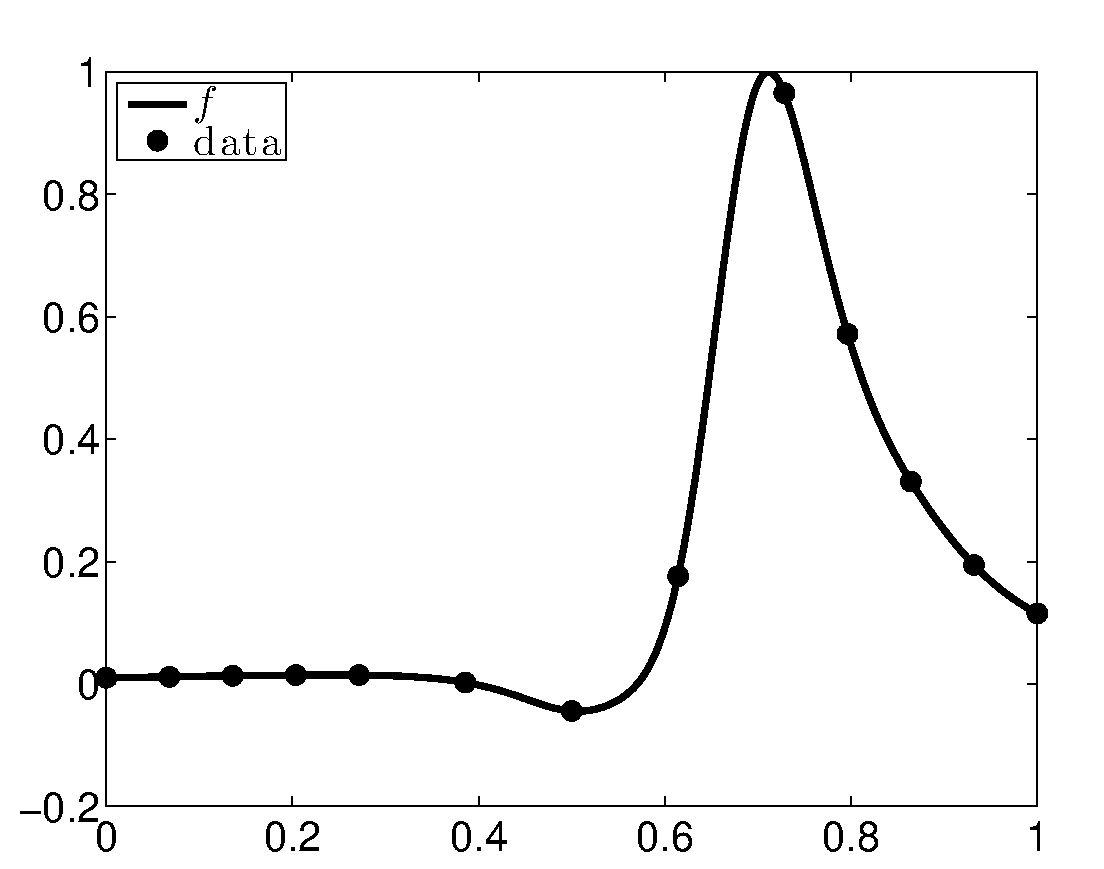
\includegraphics[width=8cm]{foolbwquadexample.eps}
\caption{Integrand designed to fool MATLAB's {\tt quad} along with the data used by {\tt quad}. \label{fig:foolquad}}
\end{figure}

While Lyness's argument is correct, it does not apply to the algorithms proposed in this article because their stopping criteria are not based on  $A_{n_{i}}(f)-A_{n_{i-1}}(f)$.  Algorithm \ref{multistageintegalgo} presented in Section \ref{integsec}, always succeeds for ``reasonable'' integrands because such integrands lie in the cone $\cc_{\tau}$.  The analogous statement is true for function approximation Algorithm \ref{multistageapproalgo}, as well as for the general Algorithms \ref{twostagedetalgo} and \ref{multistagealgo}.  All of these algorithms succeed for reasonable input functions.  

Lyness's warning in \cite{Lyn83} should not be interpreted as an objection to automatic algorithms.  It is a valid objection to stopping criteria that are based on the value of a single functional, in this case, $A_{n_{i}}-A_{n_{i-1}}$.  What Lyness clearly demonstrates is that it one may easily make a functional vanish even though the error of the algorithm is significant.

\subsection{No Advantage in Adaption}

There are rigorous results from information based complexity theory, e.g., \citep[Chapter 4, Theorem 5.2.1]{TraWasWoz88}, stating that adaption does not help, namely adaptive algorithms have no significant advantage over non-adaptive algorithms. The automatic algorithms presented here are by definition adaptive in determining the total number of function data required based on an initial sample of the input function.  The reason that adaption can help in this context is that the cone, $\cc_{\tau}$, of input functions is not a convex set.  This violates one of the assumptions required to prove the negative result that adaption does not help.

To see why $\cc_{\tau}$ is not convex, let $f_{\text{in}}$ and $f_{\text{out}}$ be functions in $\cf$ with nonzero $\cg$-semi-norms, where $f_{\text{in}}$  lies in the interior of this cone, and $f_{\text{out}}$ lies outside the cone.  This means that 
\[
\frac{\norm[\cf]{f_{\text{in}}}} {\norm[\cg]{f_{\text{in}}}} = \tau_{\text{in}} < \tau < \tau_{\text{out}} =  \frac{\norm[\cf]{f_{\text{out}}}} {\norm[\cg]{f_{\text{out}}}}.
\]
Next define two functions in terms of $f_{\text{in}}$ and $f_{\text{out}}$ as follows:
\[
f_{\pm} = (\tau-\tau_{\text{in}}) \norm[\cg]{f_{\text{in}}} f_{\text{out}}  \pm (\tau + \tau_{\text{out}}) \norm[\cg]{f_{\text{out}}} f_{\text{in}},
\]
These functions must lie inside  $\cc_{\tau}$ because
\begin{align*}
\frac{\norm[\cf]{f_{\pm}}} {\norm[\cg]{f_{\pm}}} 
&= \frac{\Bigl \lVert (\tau-\tau_{\text{in}}) \norm[\cg]{f_{\text{in}}} f_{\text{out}}  \pm (\tau + \tau_{\text{out}}) \norm[\cg]{f_{\text{out}}} f_{\text{in}}\Bigr \rVert_{\cf}}
{\Bigl \lVert (\tau-\tau_{\text{in}}) \norm[\cg]{f_{\text{in}}} f_{\text{out}}  \pm (\tau + \tau_{\text{out}}) \norm[\cg]{f_{\text{out}}} f_{\text{in}}\Bigr \rVert_{\cg}}\\
& \le 
\frac{(\tau-\tau_{\text{in}}) \norm[\cg]{f_{\text{in}}} \norm[\cf]{f_{\text{out}}}  + (\tau + \tau_{\text{out}}) \norm[\cg]{f_{\text{out}}} \norm[\cf]{f_{\text{in}}}}
{-(\tau-\tau_{\text{in}}) \norm[\cg]{f_{\text{in}}} \norm[\cg]{f_{\text{out}}}  + (\tau + \tau_{\text{out}}) \norm[\cg]{f_{\text{out}}} \norm[\cg]{f_{\text{in}}}}\\
& =
\frac{(\tau-\tau_{\text{in}})\tau_{\text{out}}  + (\tau + \tau_{\text{out}}) \tau_{\text{in}} } {-(\tau-\tau_{\text{in}}) + (\tau_{\text{out}}-\tau)}
=
\frac{\tau (\tau_{\text{out}} +\tau_{\text{in}}) } {\tau_{\text{out}} + \tau_{\text{in}}} =  \tau.
\end{align*}
On the other hand, the average of $f_{\pm}$, which is also a convex combination is 
\[
\frac{1}{2} f_- + \frac{1}{2} f_+ = (\tau-\tau_{\text{in}}) \norm[\cg]{f_{\text{in}}} f_{\text{out}}.
\]
Since $\tau > \tau_{\text{in}}$, this is a nonzero multiple of $f_{\text{out}}$, and it lies outside $\cc_{\tau}$.  Thus, this cone is not a convex set.


\section{Further Work} \label{furthersec}

The results presented here suggest a number of other interesting open problems.  Here is a summary.

\begin{itemize}

\item The univariate integration and function approximation algorithms in Sections \ref{integsec} and \ref{approxsec} have low order convergence.  Guaranteed automatic algorithms with higher order convergence rates for smoother input functions are needed.  These might be based on higher degree piecewise polynomial approximations.

\item There are other types of problems, e.g., differential equations and nonlinear optimization, which fit the general framework presented here.  These problems also have automatic algorithms, but without guarantees.  It would be helpful to develop guaranteed automatic algorithms in these other areas.

\item The algorithms developed here are \emph{globally adaptive}, in the sense that the function data determines the sample size, but not the kinds of data collected or the locations of the sample points, which depend only on the sample size.  Some existing automatic algorithms are \emph{locally adaptive} in that they collect more data in regions of special interest, say where the function has a spike.  Such algorithms need guarantees lie the ones that are provided here for globally adaptive algorithms.  The appropriate kinds of spaces $\cg$ and $\cf$, and their semi-norms, need to be identified for locally adaptive algorithms.

\item For some numerical problems the error bound of the non-adaptive algorithm involves a $\cg$- or $\cf$-semi-norm that is very hard to approximate because of its complexity.  An example is multivariate quadrature using quasi-Monte Carlo algorithms, where the error depends on the \emph{variation} of the integrand.  The definition of the variation may vary somewhat with the definition of $\cg$ or $\cf$, but it is essentially some norm of a mixed partial derivative of the integrand.  To obtain guaranteed automatic algorithms one must either find an efficient way to approximate the variation of the function or find other suitable conservative estimates for the error that can be reliably obtained from the function data.  

\item This article considers only the worst case error of deterministic algorithms.  There are many random algorithms, and they must be analyzed by somewhat different methods.  A guaranteed Monte Carlo algorithm for estimating the mean of a random variable, which includes multivariate integration as a special case, has been proposed in \cite{HicEtal14a}.

\end{itemize}

\section*{References}
\bibliographystyle{model1b-num-names.bst}
%\bibliographystyle{elsarticle-num-names}
\bibliography{FJH22,FJHown22}
\end{document}

